%%% The main file. It contains definitions of basic parameters and includes all other parts.

%% Settings for single-side (simplex) printing
% Margins: left 40mm, right 25mm, top and bottom 25mm
% (but beware, LaTeX adds 1in implicitly)
\documentclass[12pt,a4paper]{report}
\setlength\textwidth{145mm}
\setlength\textheight{247mm}
\setlength\oddsidemargin{15mm}
\setlength\evensidemargin{15mm}
\setlength\topmargin{0mm}
\setlength\headsep{0mm}
\setlength\headheight{0mm}
% \openright makes the following text appear on a right-hand page
\let\openright=\clearpage

%% Character encoding: usually latin2, cp1250 or utf8:
\usepackage[utf8]{inputenc}

%% Further useful packages (included in most LaTeX distributions)
\usepackage{amsmath}        % extensions for typesetting of math
\usepackage{amsfonts}       % math fonts
\usepackage{amsthm}         % theorems, definitions, etc.
\usepackage{bbding}         % various symbols (squares, asterisks, scissors, ...)
\usepackage{bm}             % boldface symbols (\bm)
\usepackage{graphicx}       % embedding of pictures
\usepackage{fancyvrb}       % improved verbatim environment
\usepackage{natbib}         % citation style AUTHOR (YEAR), or AUTHOR [NUMBER]
\usepackage[nottoc]{tocbibind} % makes sure that bibliography and the lists
			    % of figures/tables are included in the table
			    % of contents
\usepackage{dcolumn}        % improved alignment of table columns
\usepackage{booktabs}       % improved horizontal lines in tables
\usepackage{paralist}       % improved enumerate and itemize
\usepackage[usenames]{xcolor}  % typesetting in color
%\usepackage{lineno}

% Definitions of macros (see description inside)
%%% This file contains definitions of various useful macros and environments %%%
%%% Please add more macros here instead of cluttering other files with them. %%%

%%% Minor tweaks of style

% These macros employ a little dirty trick to convince LaTeX to typeset
% chapter headings sanely, without lots of empty space above them.
% Feel free to ignore.
\makeatletter
\def\@makechapterhead#1{
  {\parindent \z@ \raggedright \normalfont
   \Huge\bfseries \thechapter. #1
   \par\nobreak
   \vskip 20\p@
}}
\def\@makeschapterhead#1{
  {\parindent \z@ \raggedright \normalfont
   \Huge\bfseries #1
   \par\nobreak
   \vskip 20\p@
}}
\makeatother

% This macro defines a chapter, which is not numbered, but is included
% in the table of contents.
\def\chapwithtoc#1{
\chapter*{#1}
\addcontentsline{toc}{chapter}{#1}
}

% Draw black "slugs" whenever a line overflows, so that we can spot it easily.
\overfullrule=1mm

%%% Macros for definitions, theorems, claims, examples, ... (requires amsthm package)

\theoremstyle{plain}
\newtheorem{thm}{Theorem}
\newtheorem{lemma}[thm]{Lemma}
\newtheorem{claim}[thm]{Claim}
\newtheorem{obs}[thm]{Observation}
\newtheorem{fct}[thm]{Fact}

\theoremstyle{definition}
\newtheorem{defn}{Definition}
\newtheorem{ntn}{Notation}

\theoremstyle{remark}
\newtheorem*{cor}{Corollary}
\newtheorem*{rem}{Remark}
\newtheorem*{example}{Example}

%%% An environment for proofs

%%% FIXME %%% \newenvironment{proof}{
%%% FIXME %%%   \par\medskip\noindent
%%% FIXME %%%   \textit{Proof}.
%%% FIXME %%% }{
%%% FIXME %%% \newline
%%% FIXME %%% \rightline{$\square$}  % or \SquareCastShadowBottomRight from bbding package
%%% FIXME %%% }

%%% An environment for typesetting of program code and input/output
%%% of programs. (Requires the fancyvrb package -- fancy verbatim.)

\DefineVerbatimEnvironment{code}{Verbatim}{fontsize=\small, frame=single}

%%% The field of all real and natural numbers
\newcommand{\R}{\mathbb{R}}
\newcommand{\N}{\mathbb{N}}

%%% Useful operators for statistics and probability
\DeclareMathOperator{\pr}{\textsf{P}}
\DeclareMathOperator{\E}{\textsf{E}\,}
\DeclareMathOperator{\var}{\textrm{var}}
\DeclareMathOperator{\sd}{\textrm{sd}}

%%% Transposition of a vector/matrix
\newcommand{\T}[1]{#1^\top}

%%% Various math goodies
\newcommand{\goto}{\rightarrow}
\newcommand{\gotop}{\stackrel{P}{\longrightarrow}}
\newcommand{\maon}[1]{o(n^{#1})}
\newcommand{\abs}[1]{\left|{#1}\right|}
\newcommand{\dint}{\int_0^\tau\!\!\int_0^\tau}
\newcommand{\isqr}[1]{\frac{1}{\sqrt{#1}}}

%%% Various table goodies
\newcommand{\pulrad}[1]{\raisebox{1.5ex}[0pt]{#1}}
\newcommand{\mc}[1]{\multicolumn{1}{c}{#1}}


\begin{document}
%\linenumbers

\chapter{Introduction}
\textbf{TODO}:
\begin{itemize}
	\item Fix or rewrite Lemma~\ref{lemma:maxmult}.
	\item Consider adding more patterns/generalizations.
	\item Figure out what to do with Theorem 4.31.
	\item Consider fixing Lemma 4.33 (currently commented).
\end{itemize}

A binary matrix (or 0--1 matrix) is a matrix with ones and zeroes as its entries. In the thesis, we only consider binary matrices and so we omit the word binary. We say that a matrix~$M$ contains a matrix~$P$ as an interval minor, if $P$ can be created from $M$ by a sequence of deletion of one-entries and merges of neighboring rows or columns. Otherwise, we say $M$ avoids $P$. To distinguish among matrices and to indicate the relationship, we usually call the matrix~$P$ a \emph{pattern}.

When working with matrices, we always index rows from top to bottom and columns from left to right, starting with one. When we speak about a row~$r$, we mean a row with index $r$. A \emph{line} of a matrix is either a row or a column.

\section{The main results}
While a lot is know about matrices in general, because they can intuitively represent much more complex objects, interval minors are a fairly new topic and so we have a choice of the direction from which we want to approach them.

To get familiar with definitions and pattern avoidance in general, in Chapter~\ref{chap:chars}, we focus on small patterns (having up to four one-entries only) and describe the common structure of matrices avoiding them.

We then turn our focus elsewhere in Chapter~\ref{chap:ops}, and instead of looking for a structure of matrices avoiding a pattern, given a class of matrices (closed under interval minors) we find the smallest set of forbidden patterns that characterizes the class. We introduce the skew sum of two matrices and show that classes of matrices closed under the skew sum can always be described by a finite number of forbidden pattern. Using the operation more, we show that there are also other classes for which this cannot be achieved.

Because it is very useful to study extremal questions like the maximum number of one-entries of a matrix from a given class of matrices, in Chapter~\ref{chap:ints}, we study a variant of such complexity question, where we instead focus on the maximum number~$k$ of appearances of pairs ``01'' and ``10'' on a single line of a matrix from a given class of matrices. We show that even for classes that are described by just one forbidden pattern, $k$ can be unbounded, and we characterize exactly for which pattern this holds. Then we generalize the approach and show what influence an intersection of classes has on the number $k$.

\section{Preliminaries}
\begin{ntn}
For $n\in\mathbb{N}$, let $[n]:=\{1,2,\dots,n\}$ and for $m\in\mathbb{N}$ such that $n\leq m$, let $[n,m]:=\{n,n+1,\dots,m\}$.
\end{ntn}

\begin{ntn}
For a matrix~$M\in\Mat$, $R\subseteq[m]$ and $C\subseteq[n]$, let $M[R,C]$ denote a submatrix of $M$ induced by row indices in $R$ and column indices in $C$. Furthermore, for $r\in[m]$ and $c\in[n]$, let $M[r,c]:=M[\{r\},\{c\}]$.
\end{ntn}

The pattern avoidance for matrices is a generalization of a long studied theory of pattern avoidance for permutations. There are two generally used ways to define this generalization, either we avoid a matrix pattern as a submatrix or as an interval minor. While this thesis works almost exclusively with the latter, to better introduce the whole area, we start by defining the more know of the two approaches.

\begin{defn}
We say a matrix~$M\in\Mat$ \emph{contains} a pattern~$P\in\Pat$ \emph{as a submatrix} and denote it by $\PsmM$ if there are $R\subseteq[m]$ and $C\subseteq[n]$ such that $M'=M[R,C]\in\Pat$ and for every $r\in R$ and $c\in C$, if $P[r,c]=1$ then $M'[r,c]=1$.
\end{defn}

Every matrix~$M\in\Mat$ can be looked at as an adjacency matrix of a bipartite graph $G_M$ with two sets of vertices $V_1=[m]$ and $V_2=[n]$ such that a vertex~$i$ from $V_1$ is adjacent to a vertex $j$ from $V_2$ if and only if $M[i,j]=1$. The order of vertices in each set is fixed and these graphs are usually called ordered bipartite graphs. In this setting, a matrix~$M$ contains a pattern~$P$ if the ordered bipartite graph $G_P$ is a subgraph (not necessarily induced) of the ordered bipartite graph $G_M$.

In graph theory, the next step is to look at graph minors. A minor is created from a graph by a repeated applying of one of three graph operations: deletion of a vertex, deletion of an edge and a contraction of an edge. The same can be represented in terms of matrices:

\begin{defn}
We say a matrix~$M\in\Mat$ \emph{contains} a pattern~$P\in\Pat$ \emph{as an interval minor} and denote it by $\PimM$ if there is a sequence of elementary operations that applied to $M$ creates $P$. The elementary operations are:
\begin{itemize}
	\item a deletion of a line,
	\item a deletion of a one-entry (a change of a one-entry to a zero-entry) and
	\item a merge of two neighboring rows or columns into one that is the elementwise OR of the two original lines. 
\end{itemize}
\end{defn}

For simplicity, we do not consider a deletion of a line to be a separate operation as it can be replaced by a merge of the corresponding line with a neighboring one and a series of changes of one-entries to zero-entries. Moreover, like in the realm of graphs, we can assume all merging operations are done before the deletion of one-entries. This give us an alternative way to look at the problem.

\begin{defn}
Consider matrices $P$ and $M$ and let $P\im M$. A \emph{mapping} of $P$ to $M$ is a function that maps each row of $P$ to an interval of rows of $M$ and each column of $P$ to an interval of columns of $M$ in such a way that if $P[r,c]=1$ and $r$ is mapped to $R$ and $c$ is mapped to $C$, there is a one-entry in $M[R,C]$. An \emph{interval of rows} (columns) is a set of consecutive rows (columns). We say that an entry~$P[r,c]$ is mapped to an entry~$M[r',c']$ in a fixed mapping of $P$ to $M$, in which $r$ is mapped to $R$ and $c$ is mapped to $C$, if $r'\in R$ and $c'\in C$ and if $P[r,c]=1$ then we also require $M[r',c']=1$.
\end{defn}

Each mapping of a pattern~$P$ to a matrix~$M$ corresponds to a \emph{partitioning} of $M$ to intervals of rows and columns that creates a block structure. On the other hand, if we find a partitioning of $M$ to blocks such that for each one-entry $P[r,c]$ there is a one-entry in the block that can be indexed $[r,c]$ then we have a mapping of $P$ to $M$ and so $P\im M$. This means:

\begin{obs}
For all matrices $P$ and $M$, there is a mapping of $P$ to $M\Leftrightarrow\PimM$. \qed
\end{obs}

While pattern avoidance in terms of submatrices and interval minors seem to be very different, they have a quite tight relationship. The next observation immediately follows from their definitions.

\begin{obs}
\label{obs:submin}
For all matrices $P$ and $M$, $\PsmM\Rightarrow\PimM$.
\end{obs}

As said at the beginning of the section, both approaches generalize pattern avoidance for permutations and so it makes sense that they are equal for permutation matrices -- matrices having exactly one one-entry in each line.

\begin{obs}
\label{obs:perm}
For all matrices $P$ and $M$, if $P$ is a permutation matrix then $\PsmM\Leftrightarrow\PimM$.
\end{obs}
\begin{proof}
If we have $\PimM$, then there is a mapping~$m$ of $P$ to $M$. To show $P\leq M$ we need to find $R,C$ such that $M'=M[R,C]$ has the same size as $P$ and for every $P[r,c]=1$ it holds $M'[r,c]=1$. We define $R$ and $C$ as follows. For every row~$r$, let $R'$ be the interval to which $r$ is mapped in the mapping~$m$. There is exactly one column~$c$ such that $P[r,c]=1$ and $c$ is mapped to some $C'$. Because $m$ is a mapping, there is a one-entry $M[r',c']$ such that $r'\in R'$ and $c'\in C'$ and we add $r'$ to $R$ and we add $c'$ to $C$.

The other implication follows from Observation~\ref{obs:submin}.
\end{proof}

\begin{defn}
A \emph{class} of matrices~$\class{M}$ is a set of matrices that is closed under interval minors. It means that for every $M\in\class{M}$ and every $M'\im M$ it holds $M'\in\class{M}$.
\end{defn}

To avoid degenerate cases, we only consider classes of matrices containing at least one matrix of size $2\times1$, at least one matrix of size $1\times2$ and at least one matrix that is non-empty.

\begin{defn}
Let $\class{P}$ be a set of patterns. We denote by $\Avm{\class{P}}$ the set of all matrices that avoid each $P\in\class{P}$ as an interval minor.
\end{defn}

\begin{obs}
\label{obs:im}
For all patterns $P$ and $P'$: $P\im P'\Leftrightarrow\Avm{P}\subseteq\Avm{P'}$.
\end{obs}
\begin{proof}
Because $P\im P'$, every matrix that avoids $P$ also avoids $P'$. On the other hand, if $P\nim P'$ then $P'\in\Avm{P}$. As $P'\not\in\Avm{P'}$, we have $\Avm{P}\not\subseteq\Avm{P'}$.
\end{proof}

The following observation goes almost without saying and we use it throughout the whole thesis to break symmetries.

\begin{obs}
Let $P$ and $M$ be matrices, $\PimM\Leftrightarrow P^T\im M^T$.
\end{obs}

\section{Pattern avoidance}
Pattern avoidance is a general topic in combinatorics. A lot of attention is directed towards permutations, see books \cite{bona, kitaev} for references. It is a natural generalization to regard permutations as permutation matrices and consider matrix avoidance. This is mainly studied in terms of submatrices, so we discuss some interesting results in this section.

Interval minors are, on the other hand, a fairly new topic first defined by Jacob Fox in \cite{fox} as a tool to prove results about permutations in the study of Stanley--Wilf limits. Since then, a little has been discovered about the theory of interval minors. Nevertheless, we mention some results at the end of this section.

Let us go back to submatrices for now. The question that is particularly interesting is to determine the maximum number of one-entries that a matrix avoiding a given pattern can have. This property describes complexity of a pattern and can be used for example to prove algorithmic complexity, see \cite{efrat}.

\begin{defn}
Let $M$ be a matrix. The weight of $M$, denoted by $|M|$, is the number of one-entries in $M$.
\end{defn}

\begin{defn}
For a pattern~$P$ and integers $m,n$, we define the \emph{weight extremal function}~$Ex(P,m,n):=\max\{|M|;\ M\in\Mat\wedge\PnsmM\}$.
\end{defn}

Going back to the representation of the problem in terms of ordered bipartite graphs, the question to determine $Ex(P,m,n)$ is a variant of a classical Tur{\'a}n extremal graph question and was studied by many authors, see for example \cite{tardos, furedi} or, for a wider range of variants \cite{brass, claesson, klazar, pach}. Some applications associated with the weight extremal function are discussed in \cite{fulek}. There are other extremal functions that have been studied, see for instance \cite{kyncl}, but we do not consider them in this thesis.

In the same spirit, we also define the weight extremal function for matrices avoiding patterns as interval minors.

\begin{defn}
For a pattern~$P$ and integers $m,n$, we define $Ex_{\preceq}(P,m,n):=\max\{|M|;\ M\in\Mat\wedge\PnimM\}$.
\end{defn}

Thanks to Observation~\ref{obs:submin} we have the following relationship between the extremal functions.

\begin{obs}
\label{obs:exm<ex}
For all patterns~$P$ and integers $m,n$:

$Ex_{\preceq}(P,m,n)\leq Ex(P,m,n)$. \qed
\end{obs}

From Observation~\ref{obs:im} it follows:

\begin{obs}
For all patterns~$P$ and $P'$ and integers $m,n$: $P\im P'\Rightarrow Ex_{\preceq}(P,m,n)\leq Ex_{\preceq}(P',m,n)$.
\end{obs}

It was showed in \cite{Marcus} that for every permutation matrix~$P$ and every $n$ it holds $Ex(P,n,n)\leq c_Pn$. While $Ex(P,n,n)$ can become even quadratic with $n$, because of the previous observation and the fact that every pattern~$P\in\Pat$ is an interval minor of some permutation pattern~$P'\in\bin^{(kl)\times(kl)}$ we have the following:

\begin{prop}
For every pattern~$P$ and integer~$n$: $Ex_{\preceq}(P,n,n)\leq c_Pn$ for some constant $c_P$ independent of $n$. \qed
\end{prop}

The following observation for $Ex(P,m,n)$ was made by several authors; see for example \cite{cibulka09, fulek}.

\begin{lemma}
If $P\in\{0,1\}^{k\times l}$ has at least one one-entry, then

$Ex(P,m,n)\geq\Big\{\begin{array}{ll}
m\cdot n & k>m\text{ or } l>m \\
(k-1)n+(l-1)m-(k-1)(l-1) & \text{otherwise.}
\end{array}$

Moreover, the same holds for $Ex_{\preceq}(P,m,n).$
\end{lemma}
\begin{proof}
If $k>m\vee l>m$, we have $P\nim\{1\}^{m,n}$. Otherwise, let $P[r,c]=1$ and consider Figure~\ref{fig:minimalist}. Consider a matrix~$M$ such that the first $r-1$ rows, the last $k-r$ rows, the first $c-1$ column and the last $l-c$ column contain no zero-entry and the rest is empty. Then $P\not\leq M$ and even $P\nim M$. We can also see that $|M|=mn-(m-k+1)(n-l+1)=(l-1)m+(k-1)n-(k-1)(l-1)$.
\end{proof}
\begin{figure}[!ht]
\centering
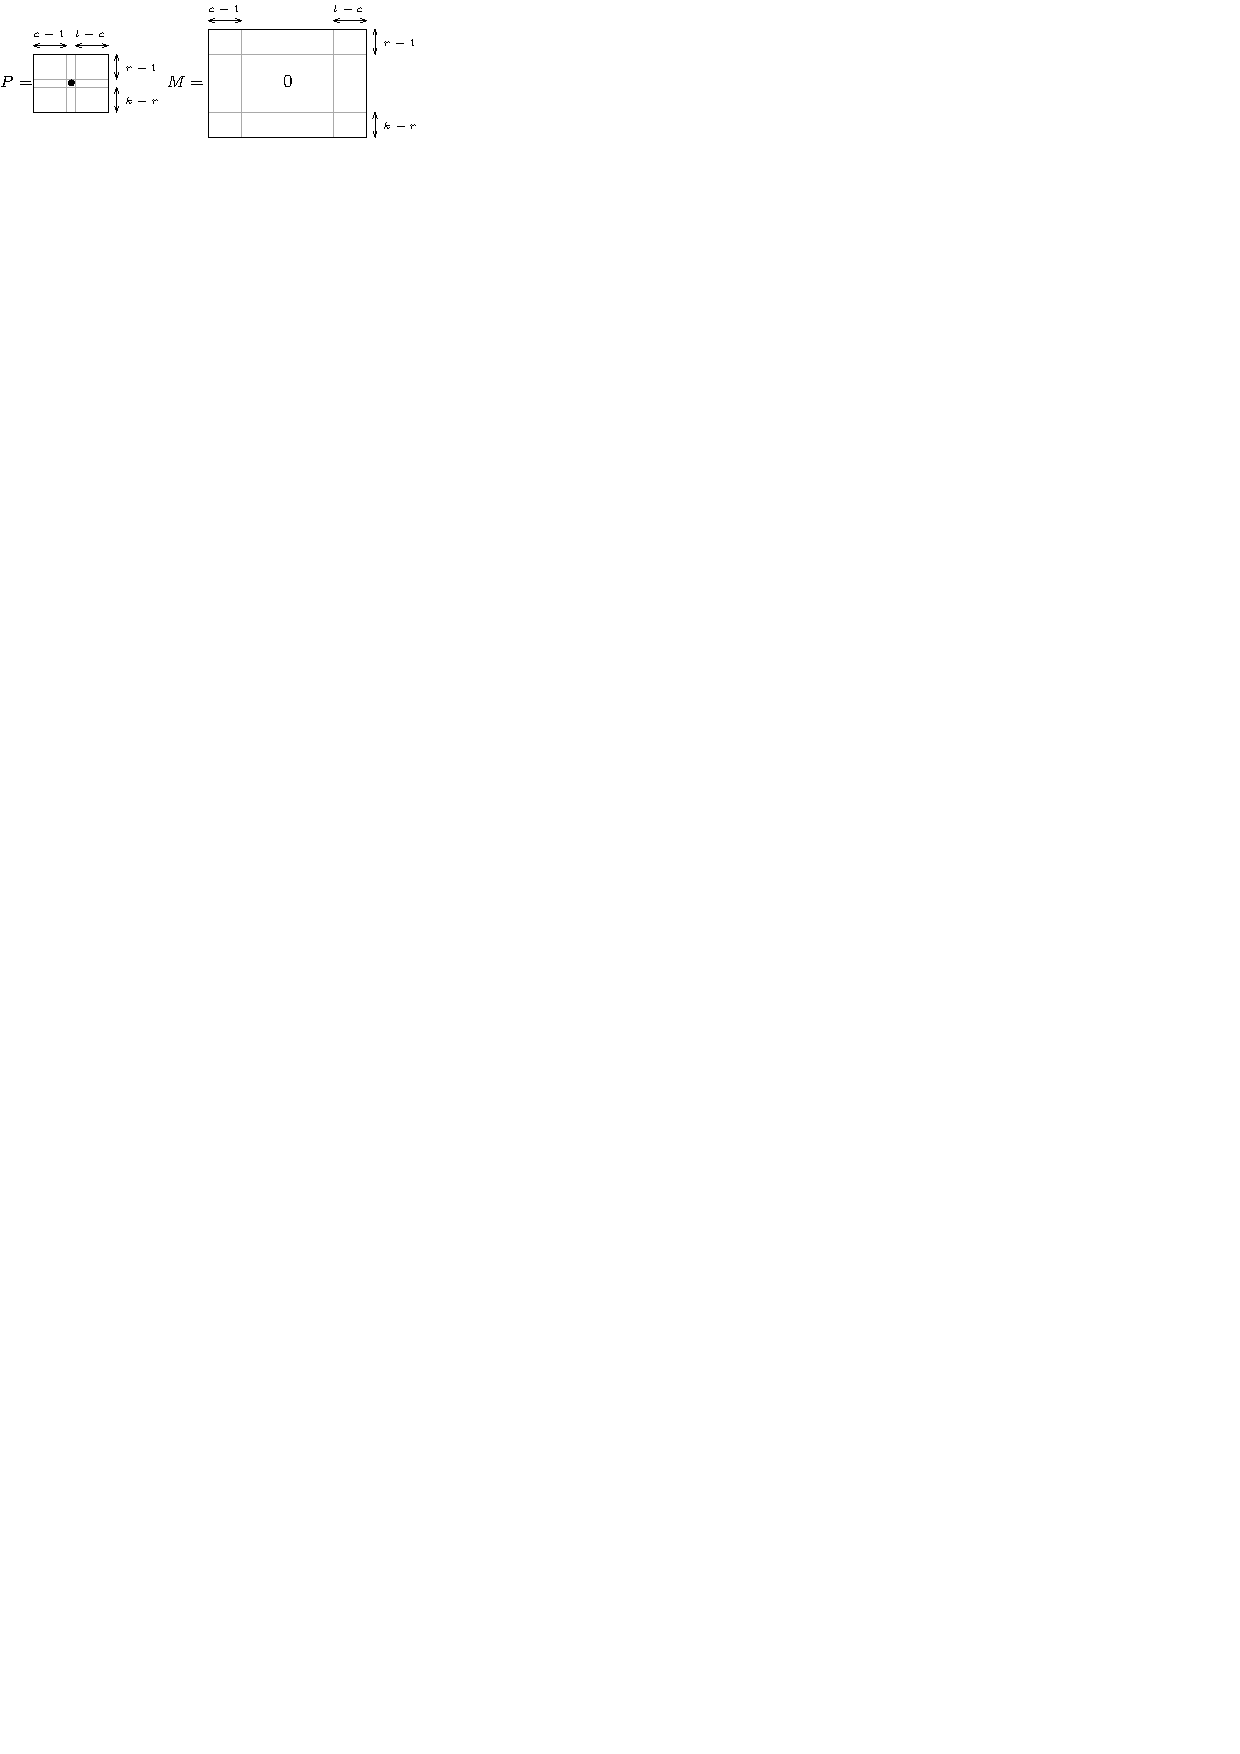
\includegraphics[width=120mm]{img/minimalist.pdf}
\caption{An example of a matrix~$M$ avoiding a pattern~$P$ as an interval minor.}
\label{fig:minimalist}
\end{figure}

The following definition is due to \cite{cibulka}.

\begin{defn}
A pattern~$P\in\{0,1\}^{k\times l}$ is \emph{(strongly) minimalist} if
$$Ex(P,m,n)=\Big\{\begin{array}{ll}
m\cdot n & k>m\text{ or } l>m \\
(k-1)n+(l-1)m-(k-1)(l-1) & \text{otherwise.}
\end{array}$$
\end{defn}

We use the adjective ``strongly'' to further distinguish minimalist pattern from weakly minimalist patterns defined next.

\begin{defn}
A pattern~$P\in\{0,1\}^{k\times l}$ is \emph{weakly minimalist} if
$$Ex_{\preceq}(P,m,n)=\Big\{\begin{array}{ll}
m\cdot n & k>m\text{ or } l>m \\
(k-1)n+(l-1)m-(k-1)(l-1) & \text{otherwise.}
\end{array}$$
\end{defn}

From Observation~\ref{obs:exm<ex}, we immediately have:

\begin{obs}
\label{obs:strongweak}
If a pattern~$P$ is strongly minimalist then $P$ is weakly minimalist.
\end{obs}

The following result is a simplification of a lemma from \cite{cibulka}.

\begin{fct}
\label{fct:minimalist}
\begin{enumerate}
	\item The pattern~$\smm{\bullet}$ is strongly minimalist.
	\item If a pattern~$P\in\Pat$ is strongly minimalist and there is a one-entry in the last row of $P$ in the $c$-th column, then $P'\in\{0,1\}^{k+1\times l}$ created from $P$ by appending as the last row a new row having a one-entry only in the $c$-th column is strongly minimalist.
	\item If a pattern~$P$ having at least two one-entries is strongly minimalist, then after changing a one-entry to a zero-entry it is still strongly minimalist.
\end{enumerate}
\end{fct}

The following two facts come from \cite{bigraphs}. In the article, a slightly different definition of an interval minor is used, so we show here the proofs in our setting.

\begin{fct}[\cite{bigraphs}]
\label{fct:2weak}
Let $P=\{1\}^{2\times l}$ be a pattern, then $P$ is weakly minimalist.
\end{fct}
\begin{proof}
Let $M\in\Mat$ be a matrix avoiding $P=\{1\}^{2\times l}$ as an interval minor and let $A_i$ be the set of column indices $j$ such that both $M[[i],\{j\}]$ and $M[[i+1,m],\{j\}]$ are non-empty. Clearly, $|A_i|\leq l-1$; otherwise, $P\preceq M$. Let $b_j$ denote the number of one-entries in the $j$-th column. Each column~$j$ of $M$ appears in at least $b_j-1$ of sets $A_i$, $1\leq i\leq m-1$. It follows that

$|M|=\sum\limits_{j=1}^nb_j=\sum\limits_{j=1}^n(b_j-1)+n\leq\sum\limits_{i=1}^{m-1}|A_i|+n\leq(l-1)(m-1)+n$.
\end{proof}

This result shows an example of a weakly minimalist matrix that is not strongly minimalist. Consider a matrix~$\smm{\bullet&\bullet\\\bullet&\bullet}$. It is, thanks to Fact~\ref{fct:2weak} weakly minimalist, but it is known due to \cite{p33} that it is not strongly minimalist.

\begin{fct}[\cite{bigraphs}]
\label{fct:3weak}
Let $P=\{1\}^{3\times l}$ be a pattern, then $P$ is weakly minimalist.
\end{fct}
\begin{proof}
Let $M\in\Mat$ be a matrix avoiding $P=\{1\}^{3\times l}$ as an interval minor and let $A_i$ be a set of column indices $j$ such that both $M[[i-1],\{j\}]$ and $M[[i+1,m],\{j\}]$ are non-empty and $M[i,j]=1$. Clearly $|A_i|\leq l-1$, otherwise $P\preceq M$. Let $b_j$ denote the number of one-entries in the $j$-th column. Each column~$j$ of $M$ (for which $b_j\geq2$) appears in exactly $b_j-2$ of sets $A_i$, $2\leq i\leq m-1$. It follows that

$|M|=\sum\limits_{j=1}^nb_j=\sum\limits_{j=1}^n(b_j-2)+2n\leq\sum\limits_{i=2}^{m-1}|A_i|+2n\leq(l-1)(m-2)+2n$.
\end{proof}

We now show that the third part of Fact~\ref{fct:minimalist} is also safe for weakly minimalist patterns.

\begin{lemma}
Let $P\in\Pat$ be a weakly minimalist pattern having at least two one-entries. Then a pattern~$P'$ created from $P$ be deletion of a one-entry is also weakly minimalist.
\end{lemma}
\begin{proof}
For contradiction, consider a matrix~$M\in\Mat$ avoiding $P'$ as an interval minor such that $|M|>(k-1)n+(l-1)m-(k-1)(l-1)$. The matrix~$M$ also avoids $P$; as otherwise, we have $P'\im P\im M$. That is a contradiction with $P$ being weakly minimalist. 
\end{proof}

As a result, we have the following corollary:

\begin{cor}
Every non-empty pattern~$P$ that has at most three rows (or columns) is weakly minimalist.
\end{cor}

In \cite{cibulka09}, the author shows that for every $k\geq1$ there is a $2k\times2k$ permutation pattern for which $Ex[P,n]\geq k^2n$. Because of Observation~\ref{obs:perm}, the same construction shows that for $k\geq2$ the patterns are not weakly minimalist. It means that the previous results cannot be easily extended. On the other hand, in \cite{multipartite} the authors show some form of generalization and also other bounds regarding interval minors and their weight extremal function.
\newsavebox{\smlmat}
\savebox{\smlmat}{$\smm{\bullet&\bullet\\\bullet& }$}
\newsavebox{\smlmatb}
\savebox{\smlmatb}{$\smm{\bullet&\bullet\\\bullet&\bullet}$}
\newsavebox{\smlmatc}
\savebox{\smlmatc}{$\smm{\bullet&\bullet&\bullet\\ &\bullet& }$}

\chapter{Characterizations}
\begin{defn}
A \emph{walk} in a matrix~$M$ is a sequence of some of its entries, beginning in the top left corner and ending in the bottom right one. If an entry $M[i,j]$ is in the sequence, the next one is either $M[i+1,j]$ or $M[i,j+1]$.
\end{defn}
\begin{defn}
We call a binary matrix~$M$ a \emph{walking matrix} if there is a walk in $M$ such that all one-entries of $M$ are contained on the walk.
\end{defn}
\begin{defn}
An \emph{extended walk of size $k\times l$} in a matrix~$M$ is a subset of some of its entries, beginning in the top left corner and ending in the bottom right one. If an entry $M[i,j]$ is in the subset there is also either $M[i+1,j]$ or $M[i,j+1]$. The size describes that no more than $k$ entries directly above each other are in the subset and no more than $l$ entries directly next to each other are in the subset. We say that an extended walk of size $k\times l$ in $M$ starts with a walk~$w$, if the extended walk is a subset of entries of $M$ that
\begin{itemize}
\item lie on $w$ or below $w$ and
\item lie on $w$ shifted by $k-1$ down and by $l-1$ to the left or above it.
\end{itemize}
\end{defn}
\begin{defn}
For $M\in\Mat$ and $r\in[m],c\in[n]$ we say $M[r,c]$ is
\begin{itemize}
\item \emph{top-left empty} if $M[[r-1],[c-1]]$ is an empty matrix,
\item \emph{top-right empty} if $M[[r-1],[c+1,n]]$ is empty,
\item \emph{bottom-left empty} if $M[[r-1],[c+1,n]]$ is empty,
\item \emph{bottom-right empty} if $M[[r-1],[c+1,n]]$ is empty.
\end{itemize}
\end{defn}

\section{Patterns of size $2\times2$ and their generalization}
\label{sec2by2}

\begin{thm}
\label{walkingthm}
Let $P=\smm{ &\bullet\\\bullet& }$, then for all $M$: $\PnimM\Leftrightarrow M$ is a walking matrix.
\end{thm}
\begin{proof}
Since $P$ is a permutation matrix, $\PnimM\Leftrightarrow\PnsmM$ and it is easy to see $\PnsmM\Leftrightarrow M$ is a walking matrix.
\end{proof}

Now consider a generalization of the pattern from above:
\begin{thm}
Let $P\in\Pat$ be a matrix having only two one-entries -- $P[1,n]$ and $P[m,1]$, then for all $M$: $\PnimM\Leftrightarrow M$ has an extended walk of size $k-1\times l-1$ containing all one-entries.
\end{thm}
\begin{proof}
\begin{itemize}
\item[$\Rightarrow$] Let $\PnimM$ and consider the left-most top-right empty elements of $M$. They necessarily form a walk $w$. For contradiction, assume there is a one-entry $e$ below the extended walk of size $k-1\times l-1$ starting with $w$. Since $e$ is below the extended walk, there is an element $e'$ - the right-most element of $M$ that is neither below $e$ nor to the right from $e$ and at the same time still below the extended walk (it is possible $e=e'$). Let $e=M[r,c]$ and notice $M[r-k,c-l]$ is part of walk $w$ and because of the choice of $e'$ neither $M[r-k-1,c-l]$ nor $M[r-k,c-l-1]$ are on the walk $w$ and $M[r-k,c-l]$ must be a one-entry; therefore, together with $e$ it forms the forbidden pattern in $M$, which is a contradiction.
\item[$\Leftarrow$] Let $M[r,c]$ be any one-entry of $M$, which then necessarily lie in the extended walk. Because the size of the walk is $k-1\times l-1$, $M[r-k+1,c-l+1]$ is top-left empty and $M[r+k-1,c+l-1]$ is bottom-right empty; therefore $e$ cannot be a part of a mapping of $P$. 
\end{itemize}
\end{proof}

\begin{thm}
\label{theorem1}
Let $P=\smm{\bullet&\bullet\\\bullet& }$, then for all $M\in\Mat$: $\PnimM\Leftrightarrow$ there exist a row~$r$ and a column~$c$ such that (see Figure~\ref{p12})
\begin{itemize}
\item $M[[r-1],[c-1]]$ is empty,
\item $M[[r-1],[c+1,n]]$ is empty,
\item $M[[r+1,m],[c-1]]$ is empty and
\item $M[[r,m],[c,n]]$ is a walking matrix.
\end{itemize}
\end{thm}
\begin{figure}[!ht]
\centering
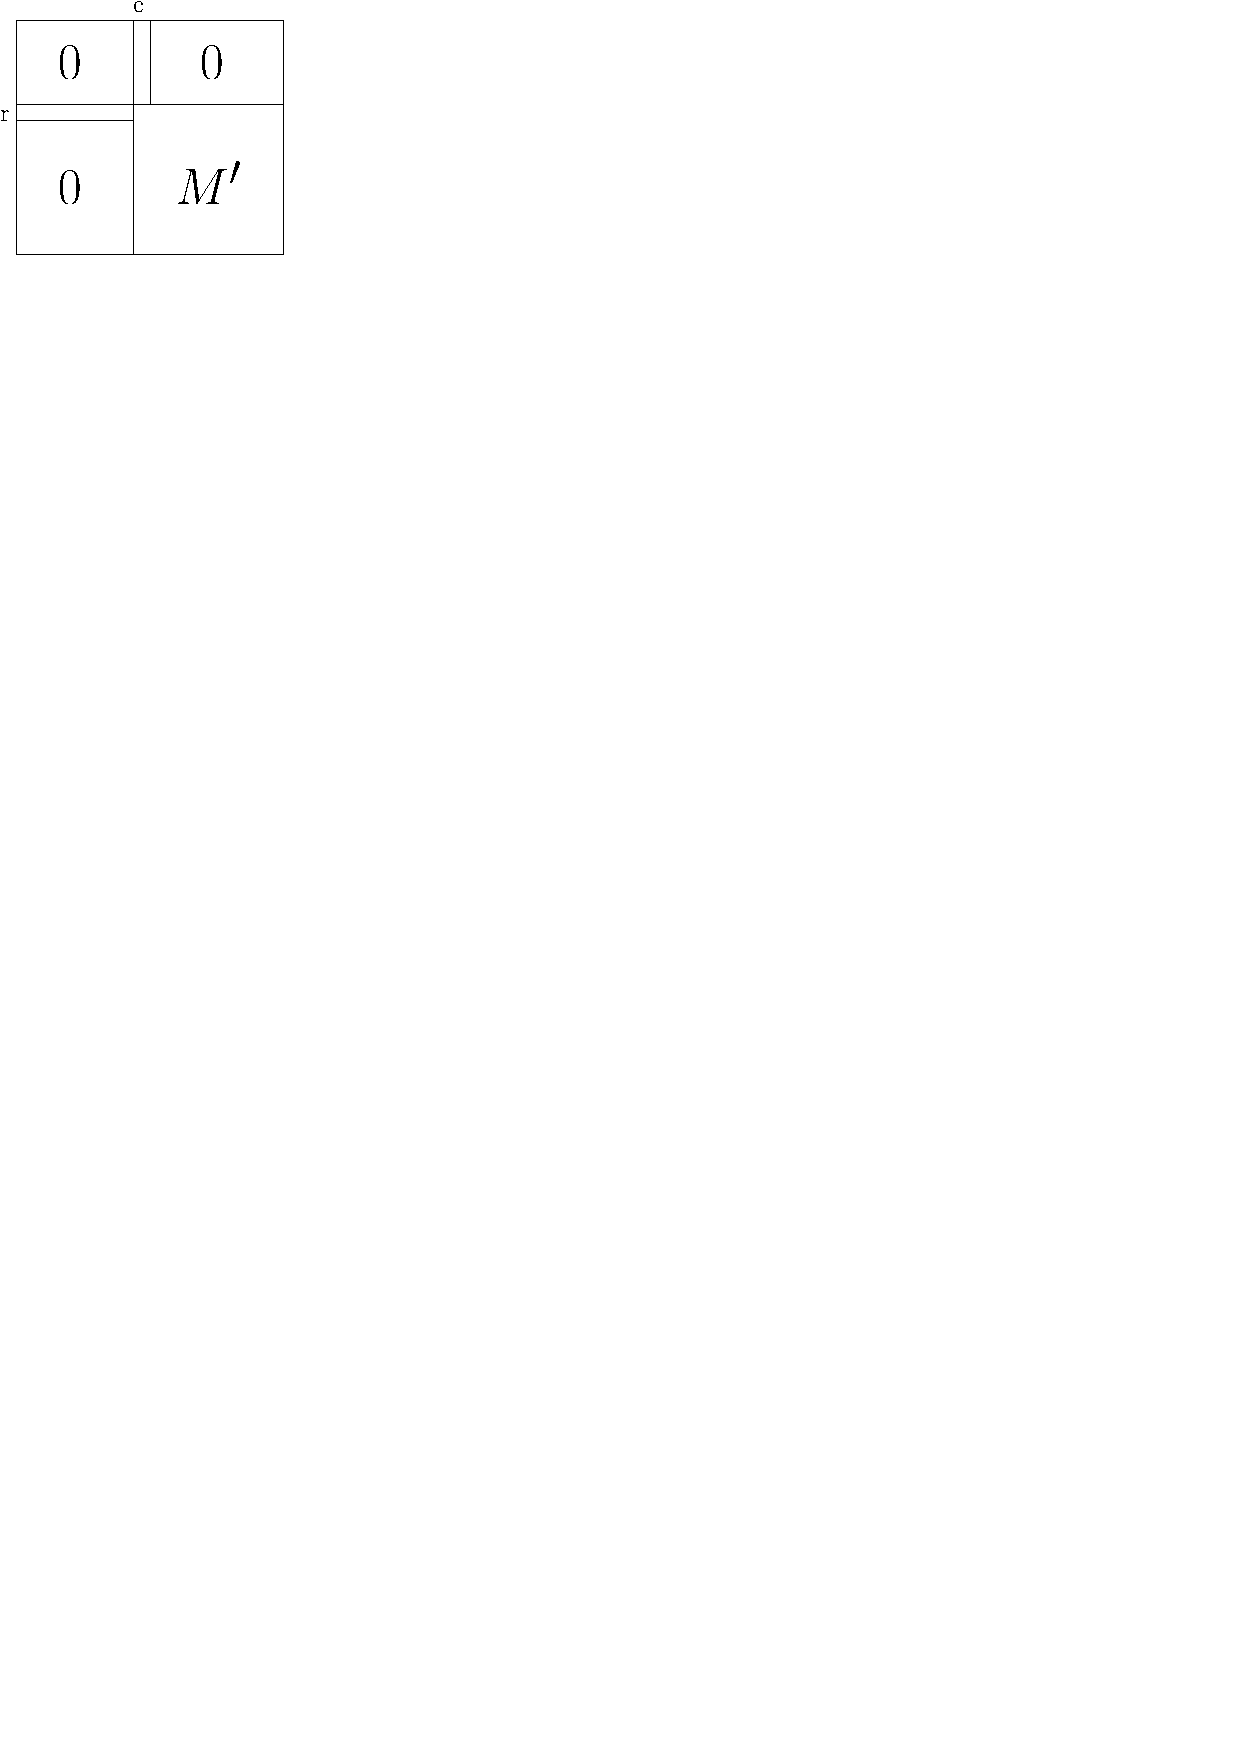
\includegraphics[width=60mm]{img/p12.pdf}
\caption{Characterization of a matrix avoiding \usebox{\smlmat} as an interval minor. Matrix $M'$ is a walking matrix}
\label{p12}
\end{figure}
\begin{proof}
\begin{itemize}
\item[$\Rightarrow$] If $\smm{ &\bullet\\\bullet& }\nim M$ then $M$ is a walking matrix and we set $r=c=1$. Otherwise, there are one-entries $M[r,c']$ and $M[r',c]$ such that $r'<r$ and $c'<c$. If there is a one-entry in regions $M[[r-1],[c-1]],\ M[[r-1],\ [c+1,n]]$ or $M[[r+1,m],[c-1]]$ then $\PimM$. If $M[[r,m],[c,n]]$ is not a walking matrix then it contains $\smm{ &\bullet\\\bullet& }$ and we again get a contradiction.
\item[$\Leftarrow$] For contradiction, assume that $M$ described in Figure~\ref{p12} contains $P$ as an interval minor. It means that there is a partition of the matrix into four quadrants such that there is at least one one-entry in each quadrant besides the bottom right one. If the matrix is partitioned above the $r$-th row, then there is only one column containing one-entries and it is not possible for both top quadrants to have a one-entry. Similarly, if the matrix is partitioned to the left of the $c$-th column, there is only one row containing one-entries and there is no one-entry in either top-left or bottom-left quadrant. Therefore, the partitioning lies bellow the $r$-th row and to the right of the $c$-th column, but if the quadrants contain one-entries, there is a $\smm{ &\bullet\\\bullet& }$ interval minor in $M'$, which is a contradiction with it being a walking matrix. % there has to be a way to write this better
\end{itemize}
\end{proof}

\begin{thm}
Let $P\in\Pat$ be a matrix having only three one-entries -- $P[1,1],\ P[1,n]$ and $P[m,1]$, then for all $M$: $\PnimM\Leftrightarrow$ there exist a row~$r$ and a column~$c$ such that (see Figure~\ref{p12} and imagine rows and columns being extended)
\begin{itemize}
\item $M[[r-1],[c-1]]$ is empty,
\item $M[[r-1],[c+l,n]]$ is empty,
\item $M[[r+k,m],[c-1]]$ is empty and
\item $M[[r,m],[c,n]]$ has an extended walk of size $k-1\times l-1$ containing all one-entries.
\end{itemize}
\end{thm}
\begin{proof} Let $P'=P$ and set $P'[m,1]=0$ ($P'$ is a generalization of $\smm{ &\bullet\\\bullet& }$). 
\begin{itemize}
\item[$\Rightarrow$] If $P'\nim M$ then $M$ is a matrix having an extended walk of size $k-1\times l-1$ containing all one-entries and we set $r=c=1$. Otherwise, there are one-entries $M[r_1,c_1]$ and $M[r_2,c_2]$ such that $r_2<r_1$ and $c_1<c_2$. We now choose $M[r_3,c_3]$ to be the bottom-most one-entry that still forms $P'$ with $M[r_2,c_2]$. We choose $M[r_4,c_4]$ to be the left-most one-entry that forms $P'$ with $M[r_3,c_3]$ and set $r=r_3-k+1$ and $c=c_4-l+1$. If there is a one-entry in regions $M[[r-1],[c-1]],\ M[[r-1],\ [c+l,n]]$ or $M[[r+k,m],[c-1]]$ then $\PimM$. If $M[[r,m],[c,n]]$ is not a walking matrix then it contains $P'$ and we again get a contradiction.
\item[$\Leftarrow$] Because of the sizes of areas with no one-entries and the condition for $M[[r,m],[c,n]]$, there cannot be $P'$ anywhere but in $M[[r+k-1],[c+l-1]]$. Since $M[[r-1][c-1]]$ is empty, there is no one-entry to map $P[1,1]$ to; therefore, $\PnimM$.
\end{itemize}
\end{proof}

\begin{lemma}
\label{lemma1}
Let $P=\smm{\bullet&\bullet\\\bullet&\bullet}$ and let $M\in\Mat$ avoid $P$ as an interval minor, then there exists a row~$r$ and a column~$c$ such that $M[r,c]$ is either
\begin{enumerate}
\item a one-entry and $(r,c)\in\{(1,1),(1,n),(m,1),(m,n)\}$ or
\item both top-left empty and bottom-right empty and $(r,c)\not\in\{(1,n),(m,1)\}$ or
\item both top-right empty and bottom-left empty and $(r,c)\not\in\{(1,1),(m,n)\}$.
\end{enumerate}
\end{lemma}
\begin{proof}
If there is a one-entry in any corner we are done. Otherwise, let $A$ be a set of all top-left empty entries of $M$ and $B$ be a set of all bottom-right empty entries of $M$. If there is an entry $M[r,c]\in A\cap B$ different from $(1,n)$ and $(m,1)$ we are done. Assume $A\cap B=\{(1,n),(m,1)\}$. Since $(m,1)\in A$, it also holds $(m-1,1)\in A$ and because it is not in the intersection we have $(m-1,1)\not\in B$. This means $M[m-1,1]$ is not bottom-right empty; therefore there is a one-entry somewhere in $M[{m},[2,n]]$. Moreover, no corner contains a one-entry so the is a one-entry in $M[{m},[2,n-1]]$. For simplicity, we will say that the last row in non-empty (knowing the corners are empty). Symmetrically, we also get that the first row is non-empty and both the first and the last columns are non-empty. If there is a one-entry $M[r_l,1]$ in a different row than a one-entry $M[r_r,n]$ and at the same time a one-entry $M[1,c_t]$ in a different column than a one-entry $M[m,c_b]$ then these four one-entries form a mapping of the forbidden pattern $P$.

This is not true!!!
%% the last statement is not true -- need to fix it, there is one more case and symmetry - will use a picture to deal with it

Without loss of generality assume there is only one one-entry in both the first and the last column and they are both in the same row $r'$. Let $c'$ be a column such that there is a one-entry $M[1,c']$. Clearly, there is no other column that contains a one-entry above $r'$, because we would again get a contradiction. Symmetrically, let $c''$ be the only column containing one-entries below $r'$. If $c'\geq c''$ we have that both $M[r',c']$ and $M[r',c'']$ are both top-left empty and bottom-right empty, which is a contradiction with $A\cap B=\{(1,n),(m,1)\}$. Otherwise, $c'<c''$ and both $M[r',c']$ and $M[r',c'']$ are both top-right empty and bottom-left empty where $(r',c')\not\in\{(1,1),(m,n)\}$ which concludes the proof.
\end{proof}

\begin{thm}
\label{t33}
Let $P=\smm{\bullet&\bullet\\\bullet&\bullet}$, then for all $M$: $\PnimM\Leftrightarrow M$ looks like one of the matrices in Figure~\ref{p33}, where $\smm{\bullet&\bullet\\\bullet& }\nim M_1$, $\smm{ &\bullet\\\bullet&\bullet}\nim M_2$, $\smm{\bullet&\bullet\\ &\bullet}\nim M_3$ and $\smm{\bullet& \\\bullet&\bullet}\nim M_4$.
\end{thm}
\begin{figure}[!ht]
\centering
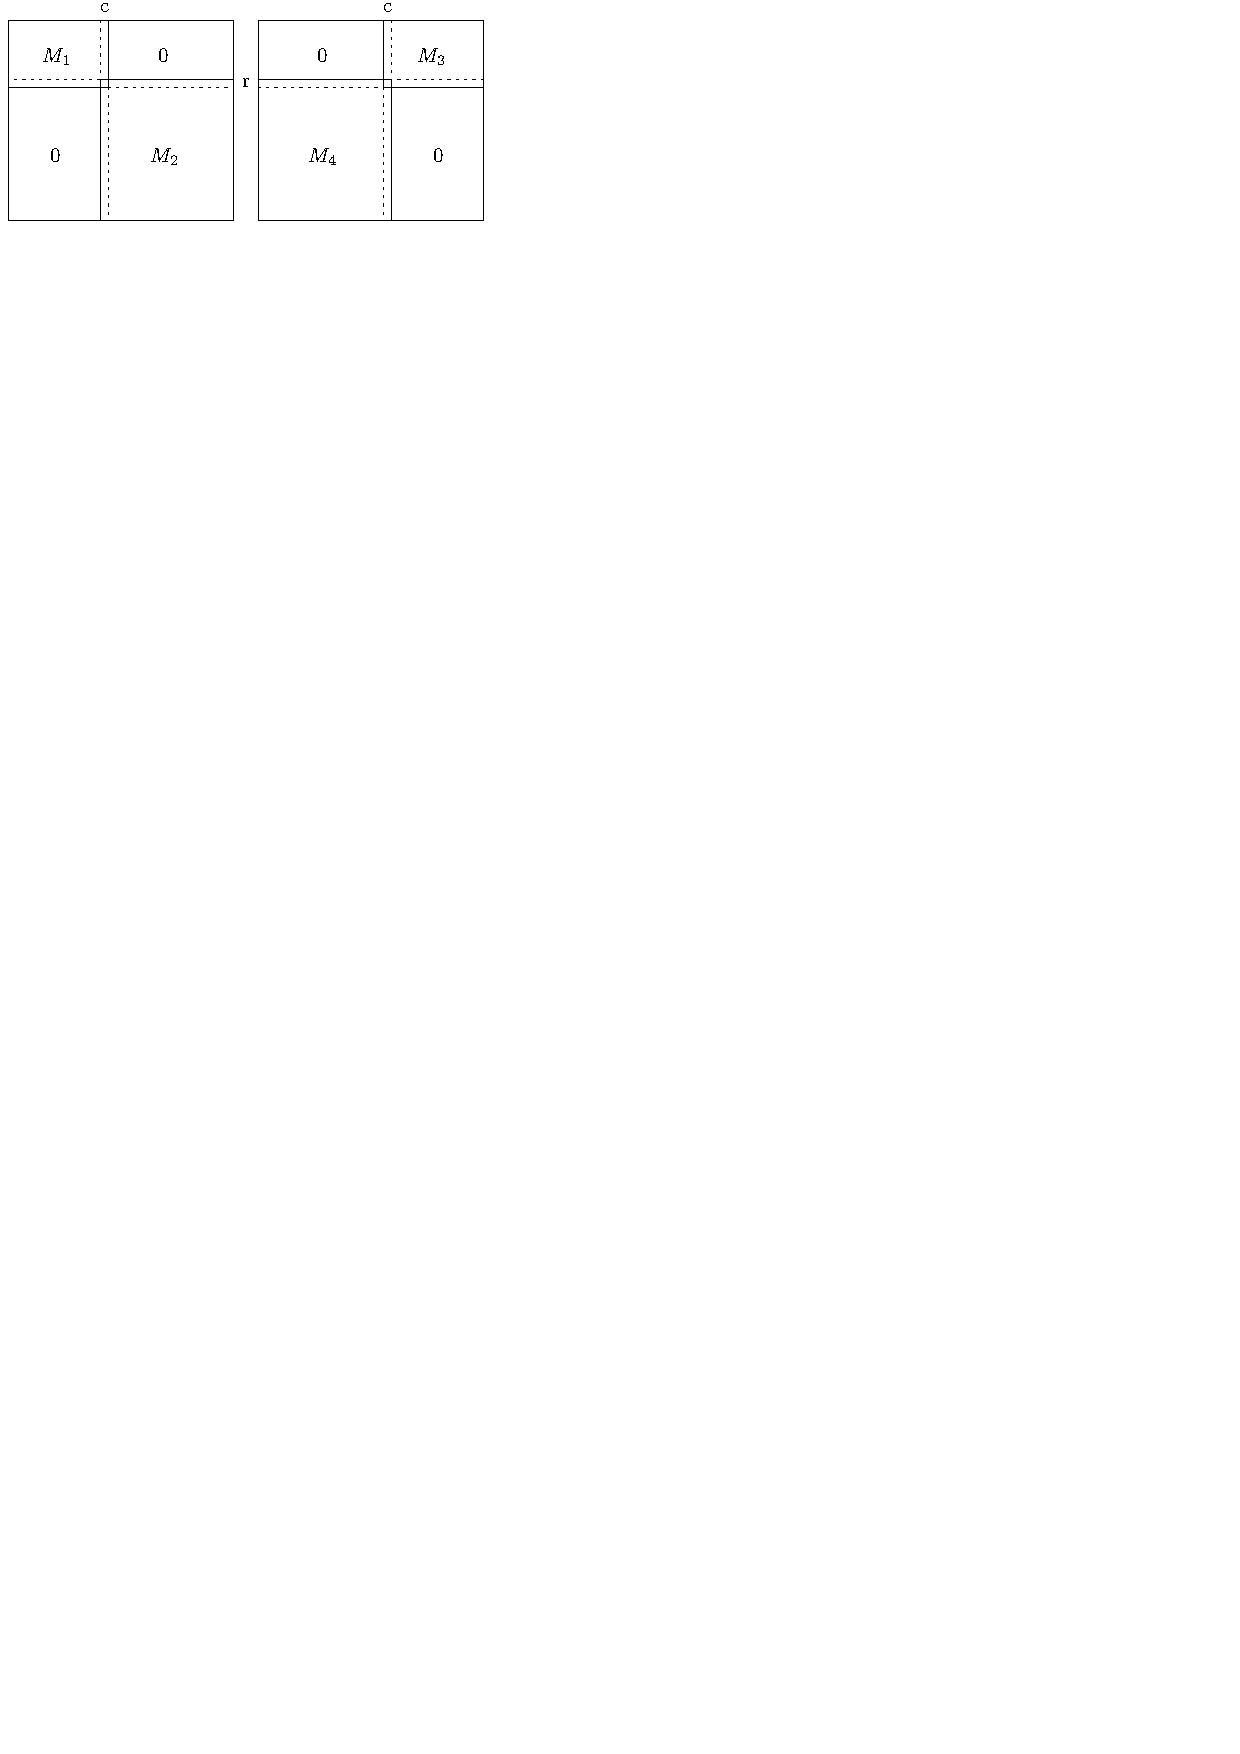
\includegraphics[height=60mm]{img/p33.pdf}
\caption{Characterization of a matrix avoiding \usebox{\smlmatb} as an interval minor.}
\label{p33}
\end{figure}
\begin{proof}
\item[$\Rightarrow$] We proceed by induction by the size of $M$.

If $M\in\{0,1\}^{2\times2}$ then it either avoids $\smm{ &\bullet\\\bullet&\bullet}$ or $\smm{\bullet&\bullet\\\bullet& }$ and we are done.

For bigger $M$ there is, from Lemma~\ref{lemma1}, $M[r,c]$ satisfying some conditions. If it is the first condition -- there is a one-entry in any corner, we are done because the matrix cannot contain one of the rotations of $\smm{\bullet&\bullet\\\bullet& }$. Assume the second case -- $M[r,c]$ is both top-right and bottom-left empty and $(r,c)\not\in\{(1,n),(m,1)\}$. If $M_1$ is non-empty, then $\smm{ &\bullet\\\bullet&\bullet}\nim M_2$; otherwise, $\PimM$. Similarly, $\smm{\bullet&\bullet\\\bullet& }\nim M_1$ if $M_2$ is non-empty. If one of them is empty, the other is a smaller matrix avoiding $P$ as an interval minor and by induction hypothesis, it can be partitioned. Adding empty rows and columns does not break any condition and we get a partitioning of the whole $M$.
\item[$\Leftarrow$] Without loss of generality, let us assume $M$ looks like the left matrix in Figure~\ref{p33}. For contradiction, assume $\PimM$. In that case, we can partition $M$ into four quadrants such that there is at least one one-entry in each of them. It does not matter where we partition it, every time we either get $\smm{\bullet&\bullet\\\bullet& }\im M_1$ or $\smm{ &\bullet\\\bullet&\bullet}\im M_2$, which is a contradiction.
\end{proof}

\begin{thm}
Let $P\in\Pat$ be a matrix having only four one-entries -- $P[1,1],\ P[1,n],\ P[m,1]$ and $P[m,n]$, then for all $M$: $\PnimM\Leftrightarrow M$ looks like one of the matrices in Figure~\ref{p33}, where generalized $\smm{\bullet&\bullet\\\bullet& }\nim M_1$, $\smm{ &\bullet\\\bullet&\bullet}\nim M_2$, $\smm{\bullet&\bullet\\ &\bullet}\nim M_3$ and $\smm{\bullet& \\\bullet&\bullet}\nim M_4$.
\end{thm}
% a lot to do here - probably will need a generalization of the lemma1

\section{Matrices of size $2\times3$}
\label{sec2by3}

\begin{thm}
Let $P=\smm{\bullet& &\bullet\\ &\bullet& }$, then for all $M$: $\PnimM\Leftrightarrow M=M_1\oplus_hM_2$ where $\smm{\bullet& \\ &\bullet}\nim M_1$ and $\smm{ &\bullet\\\bullet& }\nim M_2$.
\end{thm}
\begin{proof}
\begin{itemize}
\item[$\Rightarrow$] Let $e=[r,c]$ be the top-most one-entry of $M$. If $\smm{\bullet& \\ &\bullet}\im M[[m],[c-1]]$, together with $e$ it forms $P$. If $\smm{ &\bullet\\\bullet& }\nim M[[m],[c,n]]$ then we are done. Let us assume it is not the case and let $e_{0,0},\ e_{1,1}$ be any two one-entries forming the forbidden pattern. Symmetrically, let $\smm{\bullet& \\ &\bullet}\im M[[m],[c]]$ and let $e_{0,1},\ e_{1,0}$ be any two one-entries forming the forbidden pattern. Now if we take $e_{0,0},\ e_{0,1}$ and $e_{1,0}$ or $e_{1,1}$ with bigger row, we get the forbidden pattern $P$ as an interval minor of $M$. 
\item[$\Leftarrow$] For contradiction, let us assume $\PimM$ and $M=M_1\oplus_hM_2$. If $\PimM$, look at the one-entry of $M$ where the bottom one-entry of $P$ is mapped. If it is in $M_1$ then $\PnimM$ because $\smm{ &\bullet\\\bullet& }\nim M_1$. Otherwise, $\PnimM$ because $\smm{\bullet& \\ &\bullet}\nim M_2$.
\end{itemize}
\end{proof}

\begin{lemma}
\label{lemma2}
Let $P=\smm{\bullet&\bullet&\bullet\\ &\bullet& }$, then for all $M$: $\PnimM\Rightarrow M=M_1\oplus_hM_2$ where
\begin{enumerate}
\item $\smm{\bullet&\bullet\\ &\bullet}\nim M_1$ and $\smm{ &\bullet\\\bullet& }\nim M_2$ or
\item $\smm{\bullet& \\ &\bullet}\nim M_1$ and $\smm{\bullet&\bullet\\\bullet& }\nim M_2$.
\end{enumerate}
\end{lemma}
\begin{proof}
Let $e=[r,c]$ be the top-most one-entry of $M$. If $\smm{\bullet&\bullet\\ &\bullet}\im M[[m],[c-1]]$, together with $e$ it would be the whole $P$. Similarly, $\smm{\bullet&\bullet\\\bullet& }\nim M[[m],[c+1,n]]$. For contradiction with the statement, let $\smm{\bullet& \\ &\bullet}\im M[[m],[c]]$ and $e_{0,0},\ e_{1,1}$ (none of them equal to $e$, since $e$ lies in the top-right corner) be any two one-entries forming the pattern. Symmetrically, let $\smm{ &\bullet\\\bullet& }\im M[[m],[c,n]]$ and $e_{0,1},\ e_{1,0}$ be any two one-entries forming the pattern. In that case $e_{0,0},\ e,\ e_{0,1}$ and $e_{1,0}$ or $e_{1,1}$ with bigger row give us the forbidden pattern $P$ as an interval minor of $M$.
\end{proof}

\begin{thm}
Let $P=\smm{\bullet&\bullet&\bullet\\ &\bullet& }$, then for all $M$: $\PnimM\Leftrightarrow M$ looks like the matrix in Figure~\ref{p72} and $\smm{\bullet& \\ &\bullet}\nim M_1$ and $\smm{ &\bullet\\\bullet& }\nim M_2$.
\end{thm}
\begin{figure}[!ht]
\centering
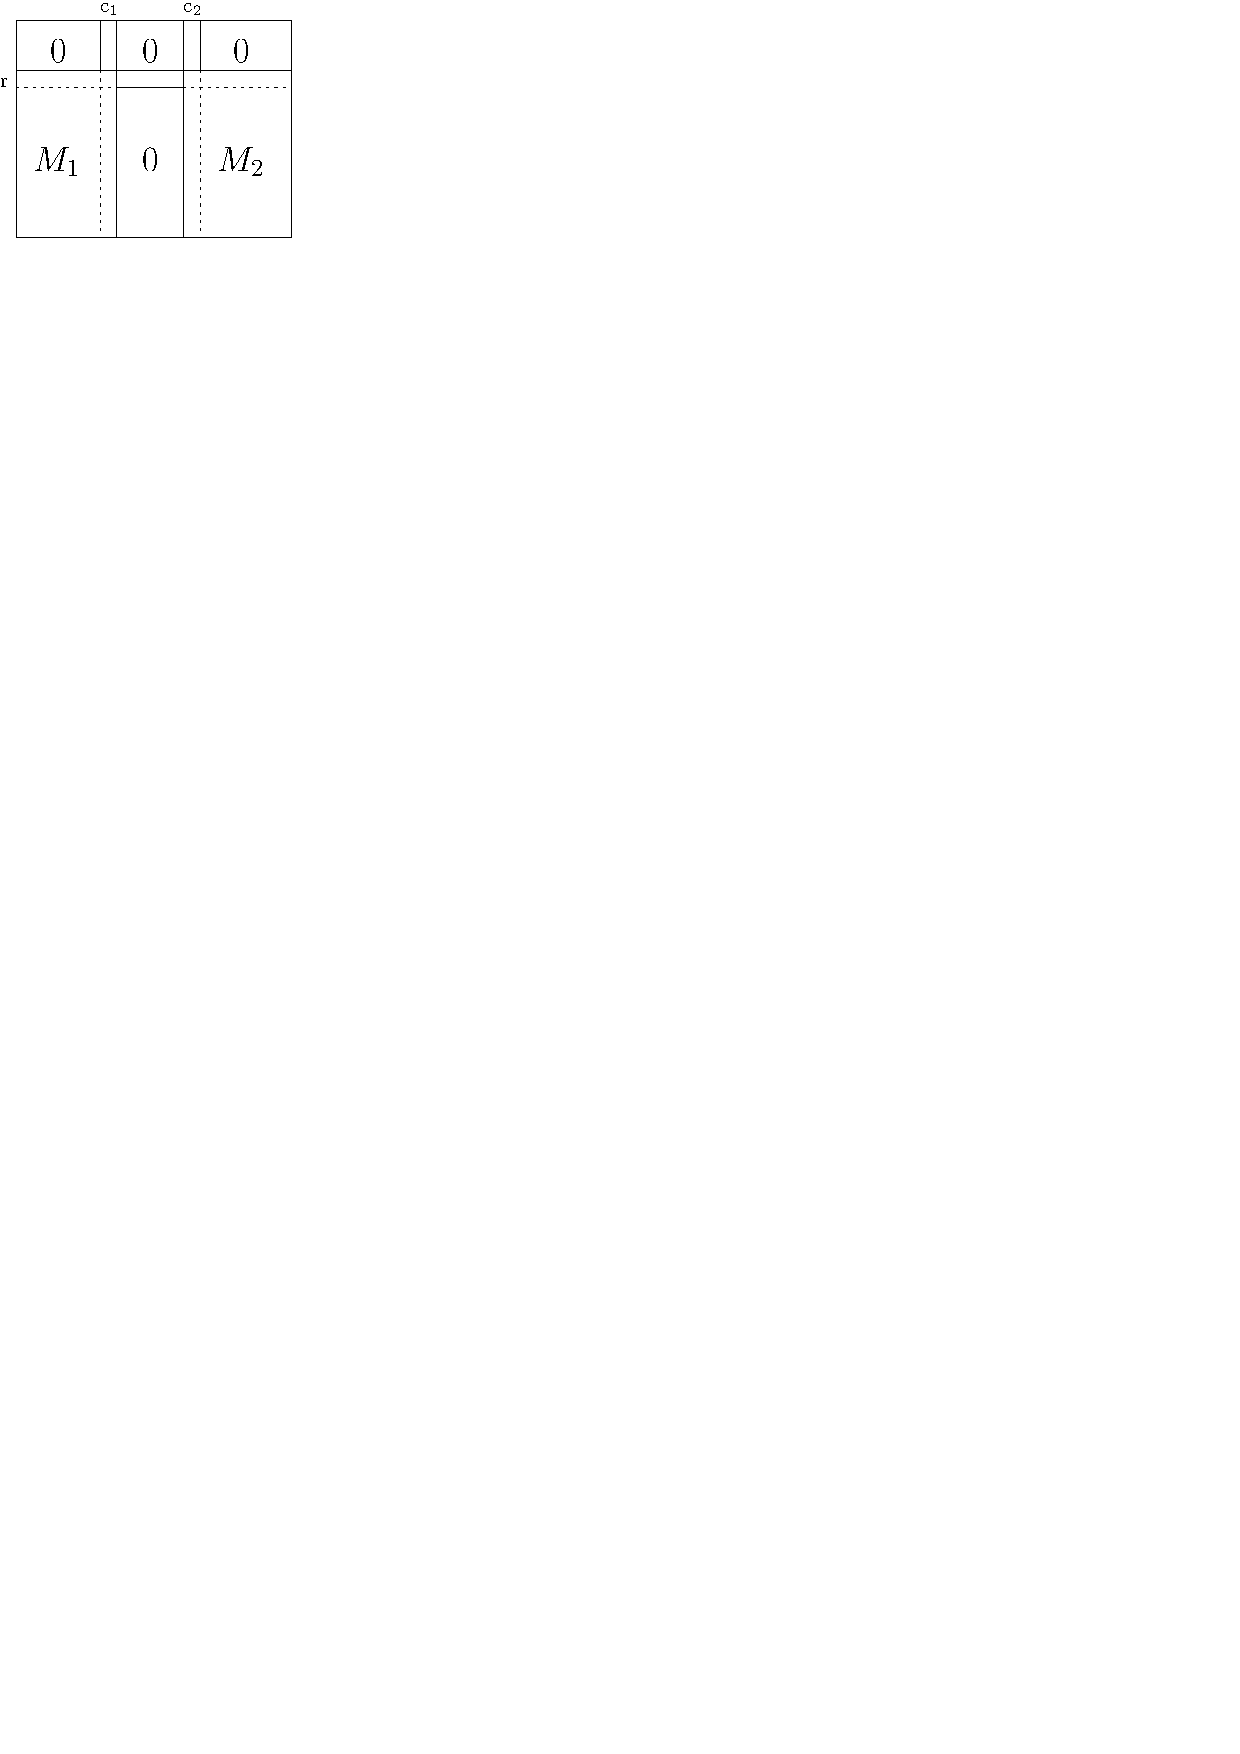
\includegraphics[height=60mm]{img/p72.pdf}
\caption{Characterization of a matrix avoiding \usebox{\smlmatc} as an interval minor.}
\label{p72}
\end{figure}
\begin{proof}
\begin{itemize}
\item[$\Rightarrow$] From Lemma~\ref{lemma2} we know $M=M_1'\oplus_hM_2'$ where $\smm{\bullet&\bullet\\ &\bullet}\nim M_1'$ and $\smm{ &\bullet\\\bullet& }\nim M_2'$. The second case would be dealt with symmetrically. From Theorem~\ref{theorem1} we have that $M_1'$ can be characterized exactly like $M[[m],[c_2-1]$ and $M[[m],[c_2,n]]$ forms a walking matrix. The only problem with our claim would be if there were two different columns having a one-entry above the $r$-th row. In that case, those two one-entries together with a one-entry in the $r$-th row between the columns $c_1$ and $c_2$ and a one-entry in the $c_1$-th column above the $r$-th row form $P$ as an interval minor.
\item[$\Leftarrow$] The bottom-middle one-entry of $P$ can not be mapped anywhere but to the $r$-th row, but in that case there are at most two columns having one-entries above it. %(will do better hopefully)
\end{itemize}
\end{proof}

\begin{thm}
Let $P=\smm{ &\bullet&\bullet\\\bullet& & }$, then for all $M$: $\PnimM\Leftrightarrow M$ contains a walk $w$, no one-entries below the walk and for each entry $M[r,c]$ of the walk there is at most one non-empty column in $M[[r-1],[c+1,n]]$.
\end{thm}
\begin{proof}
\begin{itemize}
\item[$\Rightarrow$] Let $w$ be any walk containing all the top-most and right-most entries that are bottom-left empty. From the choice of $w$, there are no one-entries below it and if all $M[r,c]$, $M[r-1,c]$ and $M[r,c+1]$ are on $w$ then $M[r,c]$ is a one-entry as else $M[r,c]$ was neither top-most nor right-most bottom-left empty. As a consequence, whenever we choose $M[r,c]$ from $w$, it either is a one-entry or there is one-entry in the same row to the left of it. For contradiction let us now assume that there is an entry of the walk $M[r,c]$ for which there are two non-empty columns in $M[[r-1],[c+1,m]]$. Then a one-entry from each of those columns and a one-entry in $M[r,c]$ or to the left of it together give us $\PimM$ and consequently a contradiction. 
\item[$\Leftarrow$] For contradiction let $\PimM$. Without loss of generality we can assume that the bottom-left entry of $P$ is mapped somewhere to the walk -- to $M[r,c]$. But then $\smm{\bullet&\bullet}\im M[[r-1],[c+1,n]]$ which is a contradiction with it having one-entries in at most one column.
\end{itemize}
\end{proof}

\section{Empty rows and columns}

\begin{obs}
\label{emptyrows}
Let $P\in\Pat$ and $P'\in\{0,1\}^{k\times l+1}$ such that $P'=P\oplus_h0^{k\times1}$, similarly let $M\in\Mat$ and $M'\in\{0,1\}^{m\times n+1}$ such that $M'=M\oplus_h1^{m\times1}$, then $\PimM\Leftrightarrow P'\im M'$.
\end{obs}
\begin{proof}
\begin{itemize}
\item[$\Rightarrow$] Clearly we can map the last column of $P'$ to the last column of $M'$ and then map (using OR) $P'[[k],[l]]$ to $M'[[m],[n]]$ the same way $P$ is mapped to $M$.
\item[$\Leftarrow$] If $P'\im M$ we are done. Otherwise, the last column of $P'$ needs to be mapped to the last column of $M'$ and by deleting both from their matrix we get $P'[[k],[l]]\im M'[[m],[n]]$ which is the same as $\PimM$.
\end{itemize}
\end{proof}

The same proof can be also used for adding an empty column as the first column or an empty row as the first or the last row. Using induction we can easily show that a pattern $P'$ is avoided by a matrix $M'$ if and only if $P$ is avoided by $M$ where $P$ is derived from $P'$ by excluding all empty beginning or ending rows and columns and $M$ is derived from $M'$ by excluding the same number of beginning or ending rows and columns. Therefore, when characterizing matrices avoiding a forbidden pattern, we do not need to consider patterns having empty rows or columns on their boundary.

For the following two statements, let $P\in\{0,1\}^{k\times2}$ be a forbidden pattern and $P^+\in\{0,1\}^{k\times3}$ be the pattern created from $P$ by adding a new empty column in between the two columns of $P$.

\begin{lemma}
\label{lemmamax}
If $M\in Av(P^+)$ is inclusion maximal, then each row of $M$ is either empty or it contains exactly one one-interval of length at least 2.
\end{lemma}

\begin{thm}
\label{emptymiddle}
For all $M\in\Mat$ it holds $M\in Av(P^+)\Leftrightarrow$ there exists $N\in\{0,1\}^{m\times(n-1)}$ such that $N\in Av(P)$ is inclusion maximal and $M$ is a submatrix of $N\oplus_h0^{m\times1}$ placed over $0^{m\times1}\oplus_hN$ with an operation bitwise OR.
\end{thm}
\begin{proof}
\begin{itemize}
\item[$\Rightarrow$] It suffices to only prove the statement for $M$ that is inclusion maximal. To do so, we use Lemma~\ref{lemmamax}. It say that each row of $M$ contains either no one-entry or an interval of length at least two. From that we define $N$ to be created from $M$ by deleting the last one-entry on each row and excluding the last column. Clearly, $M$ is equal to $N\oplus_h0^{m\times1}$ placed over $0^{m\times1}\oplus_hN$ with an operation bitwise OR. If $P\im N$ then each mapping of $P$ can be extended to a mapping of $P^+$ to $M$ by ... How to say this?

TODO
\item[$\Leftarrow$] It suffices to show that $M$ that is equal to $N\oplus_h0^{m\times1}$ placed over $0^{m\times1}\oplus_hN$ with an operation bitwise OR belongs to $Av(P^+)$. For contradiction, assume it does not. Then there is mapping of $P^+$ into elements of $M$ and we can assume that one-entries of the first column of $P^+$ are mapped to those one-entries of $M$ created from $N\oplus_h0^{m\times1}$. If it was not the case and there was a one-entry mapped to a one-entry of $M$ created only from $0^{m\times1}\oplus_hN$ we can take an element directly to its left and that is created from $N\oplus_h0^{m\times1}$. Symmetrically, all one-entries of the last column of $P^+$ are mapped to one-entries created from $0^{m\times1}\oplus_hN$. ...

TODO
\end{itemize}
\end{proof}

Open questions
\begin{itemize}
\item insertion of multiple empty columns in between two columns of $k\times2$ matrix
\item insertion of an empty column in between all columns of $P$
\end{itemize}

\section{Multiple patterns}
\begin{thm}
Let $P_1=\smm{0&0&1\\1&0&0}$ and $P_2=\smm{0&1\\0&0\\1&0}$, then for all $M$: $\PnimM\wedge\PnimM\Leftrightarrow M$ contains a walk $w$ and each one-entry $e$ is either on the walk $w$ or both element directly above $e$ and directly to the right of $e$ are on the walk $w$.
\end{thm}
\begin{proof}
\begin{itemize}
\item[$\Rightarrow$] Let us take a walk $w$ containing all the left-most and bottom-most top-right empty elements of $M$. Clearly, every top-right ``corner'' entry of $w$ ($M[r,c]$ such that both $M[r+1,c]$ and $M[r,c-1]$ are on $w$) is a one-entry. Now consider for contradiction there is a one-entry anywhere but on $w$ or directly diagonally below any top-right corner of $w$. Then this one-entry together with at least one top-right corner of $w$ give us either $P_1$ or $P_2$ and thus a contradiction.
\item[$\Leftarrow$] If we take any one-entry~$e$, from the description of $M$ there is no one-entry that would create either of $P_1$ or $P_2$ with $e$.
\end{itemize}
\end{proof}
\section{Extremal function}
\begin{ntn}
Let $M$ be a matrix. We denote $|M|$ the weight of $M$, the number of one-entries in $M$.
\end{ntn}
Usually $|M|$ stands for a determinant of matrix $M$. However, in this paper we do not work with determinants at all so the notation should not lead to misunderstanding.
\begin{defn}
For a matrix $P$ we define $Ex(P,m,n):=\max\{|M||M\in\Mat,\ \PnsmM\}$. We denote $Ex(P,n):=Ex(P,n,n)$.
\end{defn}
\begin{defn}
For a matrix $P$ we define $Ex_{\preceq}(P,m,n):=max\{|M||M\in\Mat,\ \PnimM\}$. We denote $Ex_{\preceq}(P,n):=Ex_{\preceq}(P,n,n)$.
\end{defn}
\begin{obs}
For all $P,m,n$; $Ex_{\preceq}(P,m,n)\leq Ex(P,m,n)$.
\end{obs}
\begin{obs}
If $P\in\{0,1\}^{k\times l}$ has a one-entry at position $[a,b]$, then $$Ex(P,m,n)\geq\Big\{\begin{array}{ll}
m\cdot n & k>m\vee l>m \\
(k-1)n+(l-1)m-(k-1)(l-1) & \text{otherwise.}
\end{array}$$
\end{obs}
\begin{obs}
The same holds for $Ex_{\preceq}(P,m,n).$
\end{obs}
\begin{defn}
$P\in\{0,1\}^{k\times l}$ is \emph{(strongly) minimalist} if
$$Ex(P,m,n)=\Big\{\begin{array}{ll}
m\cdot n & k>m\vee l>m \\
(k-1)n+(l-1)m-(k-1)(l-1) & \text{otherwise.}
\end{array}$$
\end{defn}
\begin{defn}
$P\in\{0,1\}^{k\times l}$ is \emph{weakly minimalist} if
$$Ex_{\preceq}(P,m,n)=\Big\{\begin{array}{ll}
m\cdot n & k>m\vee l>m \\
(k-1)n+(l-1)m-(k-1)(l-1) & \text{otherwise.}
\end{array}$$
\end{defn}
\begin{obs}
If $P$ is strongly minimalist, then $P$ is weakly minimalist.
\end{obs}
\subsection{Known results}
\begin{fct}
\begin{enumerate}
\item $\smm{1}$ is strongly minimalist.
\item If $P\in\Pat$ is strongly minimalist and there is a one-entry in the last row in the $c$-th column, then $P'\in\{0,1\}^{k+1\times l}$, which is created from $P$ by adding a new row having a one-entry only in the $c$-th column, is strongly minimalist.
\item If $P$ is strongly minimalist, then after changing a one-entry into a zero-entry it is still strongly minimalist.
\end{enumerate}
\end{fct}
% TODO: cite properly Interval minors of complete bipartite graphs - Bojan Mohar, Arash Rafiey
% Maybe mention that they were working with a different approach (ordered bigraphs) and also a different definition of an interval minor (allowing transposition) but it is not a problem for us and we show the proof in our notation.
\begin{fct}
Let $P=\smm{1\dots1\\1\dots1}$ have $l$ columns, then $P$ is weakly minimalist.
\end{fct}
\begin{proof}
Let $M\in\Mat$ be a matrix avoiding $P=\{1\}^{2\times l}$ as an interval minor and $A_i=\{j\in[n]|\text{weight of }M[[i],\{j\}]>0\wedge \text{weight of }M[[i+1,m],\{j\}>0]\}$. Clearly $|A_i|\leq l-1$, otherwise $P\preceq M$. Let $b_j$ denote the number of one-entries in the $j$-th column. Each column~$j$ of $M$ appears in at least $b_j-1$ of sets $A_i$, $0\leq i\leq m-2$. It follows that
$$\text{weight of }M=\sum\limits_{j=0}^nb_j=\sum\limits_{j=0}^n(b_j-1)+n\leq\sum\limits_{i=0}^{m-2}|A_i|+n\leq(l-1)(m-1)+n$$
\end{proof}
This result is indeed very important because it shows that there are matrices like $\smm{11\\11}$, which are weakly minimalist, although it is known they are not strongly minimalist.
\begin{fct}
Let $P=\smm{1\dots1\\1\dots1\\1\dots1}$ have $l$ columns, then $P$ is weakly minimalist.
\end{fct}
\begin{proof}
Let $M\in\Mat$ be a matrix avoiding $P=\{1\}^{3\times l}$ as an interval minor and $A_i=\{j\in[n]|\text{ weight of }M[[i-1],\{j\}]>0\wedge \text{ weight of }M[[i+1,m],\{j\}>0\wedge M[i,j]\text{ one-entry}]\}$. Clearly $|A_i|\leq l-1$, otherwise $P\preceq M$. Let $b_j$ denote the number of one-entries in the $j$-th column. Each column~$j$ of $M$ (for which $b_j\geq2$) appears in exactly $b_j-2$ of sets $A_i$, $1\leq i\leq m-1$. It follows that
$$\text{weight of }M=\sum\limits_{j=0}^nb_j=\sum\limits_{j=0}^n(b_j-2)+2n\leq\sum\limits_{i=1}^{m-2}|A_i|+2n\leq(l-1)(m-2)+2n$$
\end{proof}
\chapter{Operations with matrices}


When speaking about class of matrices, unless stated otherwise, they are closed under interval minors, which means that whenever a matrix belong to a class, all its minors belong there too. All classes discussed are also non-trivial. This means, there is at least one matrix of size $2\times1$, at least one matrix of size $1\times2$ and at least one matrix is non-empty in each class.

\begin{defn}
Let $\class{M}$ be a class of matrices. The \emph{basis} of $\class{M}$ is a set of all minimal (with respect to minors) matrices $\class{P}$ such that $\class{M}=\Avm{\class{P}}$.
\end{defn}

Let us start with a few simple observations, regarding classes of matrices and their bases. 

\begin{obs}
Let $\class{M}=\Avm{\class{P}}$ for some set of matrices $\class{P}$. Then $\class{M}$ is closed under interval minors.
\end{obs}

\begin{obs}
Every finite class of matrices has a finite basis.
\end{obs}

\section{The skew and direct sums}
In the realm of permutations, the skew and direct sums are very useful operations. What follows is a direct generalization to our settings and a few simple results. More interesting statements and the relation with interval minors follow in the next section.

\begin{defn}
For matrices $A\in\Mat$ and $B\in\Pat$ we define their \emph{skew sum} as a matrix $C:=A\dsum B\in\bin^{(m+k)\times(n+l)}$ such that $C[[k+1,m+k],[n]]=A$, $C[[k],[n+1,n+l]]=B$ and the rest is empty. Symmetrically, we define their \emph{direct sum} $D:=A\odsum B\in\bin^{(m+k)\times(n+l)}$ such that $D[[m],[n]]=A$, $D[[m+1,m+k],[n+1,n+l]]=B$ and the rest is empty.
\end{defn}

Using this notation, we can very easily rewrite the results from the previous chapter. Here is an example of Proposition~\ref{prop:p31} and Proposition~\ref{prop:p33}:

\begin{prop}
$\Avm{\smm{\bullet&\bullet\\\bullet&\circ}}=\Avm{\smm{\bullet&\circ\\\circ&\circ}}\odsum\Avm{\smm{\circ&\bullet\\\bullet&\circ}}$
\end{prop}

\begin{prop}
$\Avm{\smm{\bullet&\bullet\\\bullet&\bullet}}=\left(\Avm{\smm{\bullet&\circ\\\circ&\circ}}\odsum\Avm{\smm{\circ&\bullet\\\bullet&\circ}}\odsum\Avm{\smm{\circ&\circ\\\circ&\bullet}}\right)\cup$

\hspace{54mm}$\left(\Avm{\smm{\circ&\circ\\\bullet&\circ}}\dsum\Avm{\smm{\bullet&\circ\\\circ&\bullet}}\dsum\Avm{\smm{\circ&\bullet\\\circ&\circ}}\right)$.
\end{prop}

Something, we get a great use of later is a closure under the skew sum.

\begin{defn}
For a set of matrices $\class{M}$, let $\Cl{\class{M}}$ denote a class of matrices containing each $M\in\class{M}$ and closed under the skew sum and interval minors.
\end{defn}

When speaking about graph minors, we can always imagine that the contractions of edges are done after all deletions. Similarly, an element derived from a matrix~$M$ by reapplying the skew sum and taking its interval minor can be also derived by taking an interval minor of the skew sum of an appropriate number of copies of $M$.

\begin{obs}
For every set of matrices $\class{P}$, each $M\in\Cl{\class{P}}$ is an interval minor of the skew sum of multiple copies of $P$.
\end{obs}

What follows are two simple results of the relation of closures under the skew sum and the description using interval minors that we greatly generalize in the next section.

\begin{prop}
$\Cl{\smm{\bullet&\circ\\\circ&\bullet}}=\Avm{\smm{\bullet&\circ&\circ\\\circ&\circ&\bullet},\smm{\bullet&\circ\\\circ&\circ\\\circ&\bullet}}$.
\end{prop}
\begin{proof}
The skew sum of an arbitrary number of copies of $\smm{\bullet&\circ\\\circ&\bullet}$ avoids both forbidden patterns and because the relation of being an interval minor is transitive, we have $\Cl{\smm{\bullet&\circ\\\circ&\bullet}}\subseteq\Avm{\smm{\bullet&\circ&\circ\\\circ&\circ&\bullet},\smm{\bullet&\circ\\\circ&\circ\\\circ&\bullet}}$.

From Proposition~\ref{prop:twopatterns}, for every matrix~$M\in\Avm{\smm{\bullet&\circ&\circ\\\circ&\circ&\bullet},\smm{\bullet&\circ\\\circ&\circ\\\circ&\bullet}}$, it holds that for the top-right most walk~$w$ in $M$ such that there are no one-entries underneath it, each one-entry $M[r,c]$ is either on $w$ or both $M[r+1,c]$ and $M[r,c-1]$ are on $w$. Clearly, $\smm{\bullet&\bullet\\\bullet&\bullet}$ is an interval minor of the skew sum of three copies of $\smm{\bullet&\circ\\\circ&\bullet}$ and by the skew sum of multiple copies of $\smm{\bullet&\bullet\\\bullet&\bullet}$ we can then create the whole $w$ and all one-entries outside of it. Thus, we have the other inclusion.
\end{proof}

%\begin{prop}
%$\Cl{\smm{\bullet&\circ\\\circ&\circ\\\circ&\bullet}}=\Avm{\smm{\bullet&\circ&\circ\\\circ&\circ&\bullet},\smm{\bullet&\circ\\\circ&\circ\\\circ&\circ\\\circ&\bullet},\smm{\bullet&\circ\\\bullet&\circ\\\circ&\bullet},\smm{\bullet&\circ\\\circ&\bullet\\\circ&\bullet}}$.
%\end{prop}

While it does not make sense for permutations, we can generalize the skew sum to also allow some overlap between the summed matrices.

\begin{defn}
For matrices $A\in\Mat,\ B\in\Pat$ and integers $a,b$, let a matrix~$C:=A\dsum_{a\times b}B\in\bin^{(m+k-a)\times(n+l-b)}$ such that $C[[k+1,m+k],[n]]=A$, $C[[k],[n+1,n+l]]=B$, the part that overlaps is an elementwise OR of both submatrices and the rest of $C$ is empty. We say $C$ is the \emph{skew sum with $a\times b$ overlap} of $A$ and $B$.
\end{defn}

\begin{thm}
For integers $a,b,m,n$ such that $a\leq m\leq2a$ and $b\leq n\leq2b$, let $\class{M}$ be an arbitrary set of matrices, not necessarily closed under interval minors, such that:
\begin{itemize}
	\item $\class{M}$ is closed under deletion of one-entries,
	\item $\class{M}$ is closed under the skew sum with $a\times b$ overlap and
	\item there is a $m\times n$ matrix $M\in\class{M}$,
\end{itemize}
then $\class{M}$ is also closed under the skew sum with $(2a-m)\times(2b-n)$ overlap.
\end{thm}
\begin{proof}
Given any $A,B\in\class{M}$ and a matrix~$M\in\class{M}$ such that $M\in\Mat$, let $C=A\dsum_{a\times b}M\dsum_{a\times b}B$. It has the same size as $D=A\dsum_{(2a-m)\times(2b-n)}B$, whose set of one-entries is a subset of one-entries of $C\in\class{M}$; therefore, $D\in\class{M}$.
\end{proof}

We see that already with pretty reasonable assumptions, whenever a set of matrices is closed under the skew sum with some overlap, it is also closed under the skew sum with smaller overlap. On the other hand, in general the opposite does not hold even if we work with classes of matrices.

%NOTE: originally this was here to show that while for classes closed under minors a bigger overlap always works (now this is disproved in the following observation) so the question is whether there is any point in having this here anymore.
%\begin{obs}
%There is a set of matrices $\class{M}$ closed under submatrices but not interval minors such that it is closed under the direct sum but it is not closed under the direct sum with $1\times1$ overlap.
%\end{obs}
%\begin{proof}
%Let $\class{M}$ be a class of matrices obtained by applying the direct sum to $\smm{\bullet& \\\ &\bullet}$. Clearly, it is closed under the direct sum. On the other hand, it is not closed under the direct sum with $1\times1$ overlap, as $\smm{\bullet& \\\ &\bullet}\dsum_{1\times1}\smm{\bullet& \\\ &\bullet}=\smm{ &\bullet& \\\bullet& &\bullet\\ &\bullet& }\not\in\class{C}$.
%\end{proof}

\begin{obs}
There is a class of matrices closed under the skew sum with $1\times1$ overlap that is not closed under the skew sum with $2\times2$ overlap.
\end{obs}
\begin{proof}
Let $\class{M}=\Avm{\smm{\bullet& \\ &\bullet}}$. Clearly, $\class{M}$ is hereditary and closed under the skew sum with $1\times1$ overlap. On the other hand, $\class{M}$ is not closed under the skew sum with $2\times2$ overlap, because for matrices $\smm{\bullet&\bullet\\\bullet& },\smm{ &\bullet\\\bullet&\bullet}\in\class{M}$, it holds $\smm{\bullet&\bullet\\\bullet& }\dsum_{2\times2}\smm{ &\bullet\\\bullet&\bullet}=\smm{\bullet&\bullet\\\bullet&\bullet}\not\in\class{M}$.
\end{proof}

A similar proof shows that for all $a\geq1,b>1$ there is a class of matrices closed under the skew sum with $a\times b$ overlap that is not closed under the skew sum with $(a+1)\times b$ (or $a\times(b+1)$) overlap. Luckily for us, this does not hold for $a=0$ or $b=0$:

\begin{obs}
\label{obs:0to1}
Every class of matrices closed under the skew sum is also closed under the skew sum with $1\times1$ overlap.
\end{obs}

\section{Articulations}
Our next goal is to show that whenever we have a matrix closed under the skew sum and interval minors, the obtained class has a finite basis. In order to prove it, we define and get familiar with articulations.

\begin{defn}
Let $M\in\Mat$ be a matrix. An element $M[r,c]$ is an \emph{articulation} if it is top-left empty ($M[[r-1],[c-1]]$ is empty) and bottom-right empty ($M[[r+1,m],[c+1,n]]$ is empty). We say that an articulation $M[r,c]$ is \emph{trivial} if $(r,c)\in\{(m,1),(1,n)\}$.
\end{defn}

Whenever $P\im M$, for every $M[r,c]$ there is some $P[r',c']$ that can be mapped to $M[r,c]$; therefore, the following observation shows that once there is an articulation in $M$, it also exists in $P$ and it is not necessarily trivial.

\begin{obs}
\label{obs:keep}
Let $M$ be a matrix. If there are integers $r,c$ such that $M[r,c]$ is an articulation, then for every matrix~$P$ such that $P\im M$, if $P[r',c']$ can be mapped to $M[r,c]$ then it is an articulation.
\end{obs}

\begin{obs}
\label{obs:art}
Let $P\in\Pat$ be a matrix. There are $P_1,P_2$ non-empty interval minors of $P$ such that $P=P_1\dsum_{1\times1}P_2\Leftrightarrow$ there exist integers $r,c$ such that $P[r,c]$ is an articulation and $P[[r,k],[c]],P[[r],[c,l]]$ are non-empty.
\end{obs}

\begin{obs}
\label{obs:rel}
Let $\class{P}$ be a set of matrices. There is a minimal (with respect to interval minors) matrix~$P\in\class{P}$ and there are $P_1,P_2$ non-empty interval minors of $P$ such that $P=P_1\dsum_{1\times1}P_2\Leftrightarrow\Avm{\class{P}}$ is not closed under the skew sum with $1\times1$ overlap.
\end{obs}
\begin{proof}
\begin{itemize}
	\item[$\Rightarrow$] Let $P_1\in\bin^{k_1\times l_1}$ and $P_2\in\bin^{k_2\times l_2}$. While $P\nim P_1\dsum_{1\times1}0^{k_2\times l_2}$ and $P\nim0^{k_1\times l_1}\dsum_{1\times1}P_2$, we have $P\im P_1\dsum_{1\times1}0^{k_2\times l_2}\dsum0^{k_1\times l_1}\dsum_{1\times1}P_2$.
	\item[$\Leftarrow$] If there is no minimal matrix~$P\in\class{P}$ that is the skew sum of its non-empty interval minors, we want to show it makes $\Avm{\class{P}}$ closed under the skew sum with $1\times1$ overlap. From Observation~\ref{obs:art}, for every $P\class{P}$ there are no $r,c$ that $P[r,c]$ is an articulation and $P[[r,k],[c]],P[[r],[c,l]]$ are non-empty. Let $M_1,M_2\in\Avm{P}$ be arbitrary matrices and let $M=M_1\dsum_{1\times1}M_2$. The matrix~$M$ contains a non-trivial articulation and from Observation~\ref{obs:keep} it follows $M\in\Avm{P}$ for each minimal $P\in\class{P}$; thus, $M\in\Avm{\class{P}}$.
\end{itemize}
\end{proof}

In the following, we always expect articulations to be on a reverse walk (no two articulations forming $\smm{\bullet& \\ &\bullet}$) and by a matrix between two articulations $M[r_1,c_1]$ and $M[r_2,c_2]$ we mean the matrix $M[[r_2,r_1],[c_1,c_2]]$.

\begin{lemma}
\label{lemma:artic}
Let $\class{P}$ be a set of matrices, then for all matrices $M\in\Mat$ it holds that $M\in\Cl{\class{P}}\Leftrightarrow$ there exists a sequence of articulations of $M$ on a reverse walk such that for each matrix~$M'$ in between two consecutive articulations of $M$ there exists $P\in\class{P}$ such that $M'\im\smm{1}\dsum P\dsum\smm{1}$.
\end{lemma}
\begin{proof}
\begin{itemize}
	\item[$\Rightarrow$] With Observation~\ref{obs:0to1} in mind, consider the skew sum with $1\times1$ overlap of multiple copies of elements of $\class{P}$ and let the sequence contain an articulation between each pair of consecutive copies of matrices from $P$, together with the trivial articulations~$M[m,1]$ and $M[1,n]$.
	
	Between each pair of consecutive articulations, we have a matrix from $\class{P}$ and so the statement holds. When we take an arbitrary interval minor and keep original articulations, each matrix between two consecutive articulations only contains at most one original copy of some matrix~$P\in\class{P}$, but it may happen that the bottom-left and top-right corners become one-entries even though they were zero-entries before. The matrix does not have to be an interval minor of $P$ anymore, but it is an interval minor of $\smm{1}\dsum P\dsum\smm{1}$ for the corresponding $P\in\class{P}$.
	\item[$\Leftarrow$] We can simply blow up each matrix~$M'$ between two consecutive articulation to the skew sum of three copies of the corresponding matrix $P$ and because $M'\im\smm{1}\dsum P\dsum\smm{1}\im P\dsum P\dsum P$ it holds $M\in\Cl{\class{P}}$.
\end{itemize}
\end{proof}

Finally, we show that a closure under the skew sum can always be described by a finite number of forbidden patterns.

\begin{thm}
For all matrices~$M\in\Mat$, $\Cl{M}$ has a finite basis.
\end{thm}
\begin{proof}
Let $\class{F}$ be the set of all minimal (with respect to interval minors) matrices such that $\Cl{M}=\Avm{\class{F}}$. We need to prove that $\class{F}$ is finite. Thanks to Observation~\ref{obs:0to1}, $\Avm{\class{F}}$ is closed under the direct sum with $1\times1$ overlap and from Observation~\ref{obs:rel} follows that for no $F\in\class{F}$ there are its non-empty interval minors $F_1,F_2$ such that $F=F_1\dsum{1\times1}F_2$. We denote by $\class{P}$ a set of matrices $F\in\class{F}$ such that $F$ has at most $2m+4$ rows and $2n+4$ columns. We want to show $\Cl{M}=\Avm{\class{P}}$.
\begin{itemize}
	\item[$\subseteq$] Clearly, $\class{P}$ is finite and we immediately see that $\Cl{M}\subseteq\Avm{\class{P}}$.
	\item[$\supseteq$] For contradiction, consider a minimal matrix $X\in\Avm{\class{P}}-\Cl{M}$.
There are no $X_1,X_2$ non-empty interval minors of $X$ such that $X=X_1\dsum{1\times1}X_2$; otherwise, as $X_1,X_2\in\Avm{\class{P}}$ and $X$ is the minimum matrix such that $X\not\in\Cl{M}$, we would have $X_1,X_2\in\Cl{M}$; therefore, $X\in\Cl{M}$ and a contradiction.

Without loss of generality, we assume $X\in\Pat$ has at least $2m+5$ rows. Let $X'$ denote a matrix created from $X$ by deletion of the first row. We have $X'\in\Avm{\class{P}}$ and from minimality of $X$ also $X'\in\Cl{M}$. From Lemma~\ref{lemma:artic}, there is a sequence of articulations of $X'$ on a reverse walk such that each matrix between two consecutive articulations is an interval minor of $\smm{1}\dsum M\dsum\smm{1}$. Let $X'[r,c]$ be the first articulation from the sequence (sorted by the second coordinate in ascending order) for which $c>1$. The matrix between $X'[r,c]$ and the previous articulation in the sequence is an interval minor of $\smm{1}\dsum M\dsum\smm{1}$, which also means that $c\leq n+2$. Since $X[r,c]$ is not an articulation, it must hold that $X[1,c_1]=1$ for some $c_1<c\leq n+2$. Symmetrically, let $X''$ denote a matrix created from $X$ by deletion of the last row. Following the same steps we did before, we get the last articulation $X''[r,c]$ such that $c<l$ and the observation that $c\geq l-n-1$. Since $X[r,c]$ is not an articulation, it must hold that $X[k,c_2]=1$ for some $c_2>c\geq l-n-1$.

We showed that a matrix~$Y\in\bin^{(m+1)\times2}$ such that the only one-entries are $Y[1,1]$ and $Y[m+1,2]$ is an interval minor of $X$. To reach a contradiction, it suffices to show that there is a matrix~$P\in\class{P}$ such that $P\im Y$. For contradiction, let $Y\in\Avm{\class{P}}$ and since $Y\im X$ and $X$ is minimum such that $X\not\in\Cl{M}$ it holds $Y\in\Cl{M}$. But this cannot be, because $Y$ contains no non-trivial articulation and from Observation~\ref{obs:keep}, we know that every matrix $Z\in\Cl{M}$ bigger than $m\times n$ contains at least one.
\end{itemize}
\end{proof}

\section{Basis}
We recall that the basis of a class of matrices $\class{M}$ is a set of all minimal (with respect to interval minors) matrices $\class{P}$ such that $\class{M}=\Avm{\class{P}}$. It goes without saying that it does not make sense to consider a basis of a set of matrices that is not closed under interval minors.

So far, we showed that whenever $\class{M}$ is finite, its basis is also finite. The same hold when $\class{M}=\Cl{M}$ for some $M$. We show next that, unlike in graph theory, there are classes that does not have a finite basis. Moreover, we show that even for a class $\class{M}$ with finite basis, its closure $\Cl{\class{M}}$ can have an infinite basis.

\begin{defn}
Let $P$ be a matrix. We denote by $\R{P}$ a set of all minimal (with respect to minors) matrices $P'$ such that $P\im P'$ and $P'$ is not the skew sum with $1\times1$ overlap of non-empty interval minors of $P'$. For a set of matrices $\class{P}$, let $\R{\class{P}}$ denote a set of all minimal (with respect to minors) matrices from the set $\bigcup_{P\in\class{P}}\R{P}$.
\end{defn}

\begin{thm}
\label{thm:basis}
Let $\class{M}$ and $\class{P}$ be sets of matrices such that $\class{M}=\Avm{\class{P}}$, then $\Cl{\class{M}}=\Avm{\R{\class{P}}}$.
\end{thm}
\begin{proof}
\begin{itemize}
	\item[$\subseteq$] Assume $M\not\in\Avm{\R{\class{P}}}$ and without loss of generality, because $\Cl{\class{M}}$ is hereditary, let $M$ be minimal (with respect to interval minors). It follows that $M\in\R{\class{P}}$. As such, the matrix $M$ is not a skew sum with $1\times1$ overlap of non-empty interval minors of $M$; therefore, according to Observation~\ref{obs:art}, there is no articulations $M[r,c]$ such that $M[[r,k],[c]],M[[r],[c,l]]$ are non-empty. For contradiction, assume $M\in\Cl{\class{M}}$. According to Lemma~\ref{lemma:artic} and the fact $M$ contains no non-trivial articulation, $M$ is a minor of $\smm{1}\dsum M'\dsum\smm{1}$ for some $M'\in\class{M}$. Because the trivial articulations (top-right and bottom-left corners) contain zero-entries, it even holds $M\im M'$. We also have $M\im P$ for some $P\in\class{P}$, which together give us a contradiction with $\class{M}=\Avm{\class{P}}$.
	\item[$\supseteq$] First of all, $\Avm{\R{\class{P}}}$ is closed under the skew sum with $1\times1$ overlap. For contradiction, assume there are matrices $M_1,M_2\in\Avm{\R{\class{P}}}$ but $M=M_1\dsum_{1\times1}M_2\not\in\Avm{\R{\class{P}}}$. Then there exists a matrix~$P\in\R{\class{P}}$ such that $P\im M$. Because $P$ is not a skew sum with $1\times1$ overlap of non-empty interval minors of $P$, it follows that either $P\im M_1$ or $P\im M_2$ and we have a contradiction.

It suffices to show that the inclusion holds for any $M\in\Avm{\R{\class{P}}}$ that is not a skew sum with $1\times1$ overlap of non-empty interval minors of $M$. From Observation~\ref{obs:art}, we know that $M$ does not contain any non-trivial articulation and those trivial ones are empty. Thus, $M\in\Avm{\class{P}}=\class{M}$ and so $M\in\Cl{\class{M}}$.
\end{itemize}
\end{proof}

\begin{cor}
Let $\class{M}$ and $\class{P}$ be sets of matrices such that $\class{M}=\Avm{\class{P}}$, then $\R{\class{P}}$ is the basis of $\Cl{\class{M}}$.
\end{cor}

What follows is a construction of parameterized matrices that become the main tool of finding a class of matrices with an infinite basis.

\begin{defn}
Let $Nucleus_1=\smm{\bullet}$ and for $n>1$ let $Nucleus_n\in\bin^{n\times n+1}$ be a matrix described by the examples:
\begin{center}
$Nucleus_2=\smm{\bullet&\bullet& \\ &\bullet&\bullet}\ \ 
Nucleus_3=\smm{ &\bullet&\bullet& \\\bullet& & &\bullet\\ &\bullet&\bullet& }\ \ 
Nucleus_n=\smm{ & & & & & &\bullet&\bullet& \\ & & & & &\bullet& & &\bullet\\ & & & &\bullet& & &\bullet& \\ & & &\dots& & &\bullet& & \\ & &\bullet& & &\dots& & & \\ &\bullet& & &\bullet& & & & \\\bullet& & &\bullet& & & & & \\ &\bullet&\bullet& & & & & & \\}$.
\end{center}
\end{defn}

\begin{defn}
Let $Candy_{k,n,l}$ be a matrix given by $I_k\dsum_{1\times2}Nucleus_n\dsum_{1\times2}I_l$, where $I_k,I_l$ are unit matrices of sizes $k\times k$ and $l\times l$ respectively.
\end{defn}
$Candy_{4,1,4}=\smm{
 & & &\bullet& & & \\
 & & & &\bullet& & \\
 & & & & &\bullet& \\
\bullet& & &\bullet& & &\bullet\\
 &\bullet& & & & & \\
 & &\bullet& & & & \\
 & & &\bullet& & & }$
$Candy_{4,4,4}=\smm{
 & & & & &\bullet& & & \\
 & & & & & &\bullet& & \\
 & & & & & & &\bullet& \\
 & & & & \bullet&\bullet& & &\bullet\\
 & & &\bullet& & &\bullet& & \\
 & & \bullet& & &\bullet& & & \\
\bullet& & &\bullet&\bullet& & & & \\
 &\bullet& & & & & & & \\
 & &\bullet& & & & & & \\
 & & &\bullet& & & & & }$

\begin{thm}
\label{thm:inf}
There exists a matrix $P$ for which $\R{P}$ is infinite.
\end{thm}
\begin{proof}
Let $P=Candy_{4,1,4}$. For all $n>3$ it holds $P\im Candy_{4,n,4}$ and it suffices to show that each $Candy_{4,n,4}$ is a minimal matrix (with respect to minors) that is not the skew sum of two of its non-empty interval minors. According to Observation~\ref{obs:art}, the second condition holds as $Candy_{4,n,4}$ contains no non-trivial articulation. To show it is minimal, we need to consider any matrix $M\im Candy_{4,n,4}$ and argue that either $P\nim M$ or $M$ contains an articulation.

Thanks to Observation~\ref{obs:keep}, we can only consider one minoring operation at a time. It is easy to see that when a one-entry is changed to a zero-entry, then the matrix does not belong to $\R{P}$ anymore. Consider that rows $r_1,r_2,\dots,r_k$ are chosen to be merged into one with an elementwise OR. If $r_1<4$ or $r_k>n+3$ then $P$ is no longer an interval minor of such matrix. Otherwise, the original $Candy_{4,n,4}[r_1,n-r_1+2]$ becomes an articulation. Symmetrically, the same holds for columns which concludes the proof.
\end{proof}

\begin{cor}
There exists a class of matrices $\class{M}$ having a finite basis such that $\Cl{\class{M}}$ has an infinite basis.
\end{cor}
\begin{proof}
From Theorem~\ref{thm:inf}, we have a matrix $P$ for which $\R{P}$ is infinite. Class $\class{M}=\Avm{P}$ has a finite basis. On the other hand, from Theorem~\ref{thm:basis}, we have $\Cl{\class{M}}=\Avm{\R{P}}$.
\end{proof}

\openright
\end{document}